\documentclass[a4paper, 11pt, oneside]{book}
% \usepackage[right=8cm]{geometry}
\usepackage{fontspec}
\usepackage{lmodern}
\usepackage[english,czech]{babel}
\usepackage{csquotes}
\usepackage{url}
\usepackage{todonotes}
\usepackage{xunicode}
\usepackage{graphicx}
\usepackage{tikz-qtree}
\graphicspath{ {imgs/} }

% https://github.com/michal-h21/biblatex-iso690
% unzip to ~/texmf/tex/latex and use as style=iso-*
% some possible styles: iso-authoryear, iso-numeric, iso-alphabetic

\usepackage[
   backend=biber
  % ,style=alphabetic
  ,style=iso-alphabetic
  ,sortlocale=cs_CZ
  ,autocite=footnote
  ,maxnames=2
  ,minnames=1
  ,urldate=long
  % ,spacecolon=false
  ]
  {biblatex}

% to be fixed, this is to substitute non-existen czech norm by some other similiar, but croatian is not the one we want (does it matter?)
\DeclareQuoteAlias{croatian}{czech}

% and theres something like this:
% czech quotes
% \usepackage{csquotes}
% \DeclareQuoteStyle{czech}
%   {\quotedblbase}
%   {\textquotedblleft}
%   {\textquoteleft}
%   {\textquoteright}

% \renewcommand{\uv}[1]{
%   \enquote{#1}
% }

\addbibresource{bibliografie.bib}
\renewcommand*{\labelalphaothers}{\textsuperscript{+}}

\newcommand{\td}[2][]{
	{\hskip -0.5em\todo[size=\footnotesize]{#2}}
}

% \providecommand\parencite{}
% \providecommand\textcite{}

% \renewcommand\parencite{\cite}
% \renewcommand\textcite{\cite}

\author{edison}
\title{Vizualizace sémantické sítě}

\newcommand\ex{\textsf}

\begin{document}

	\maketitle

	\newpage

	\tableofcontents

	\newpage

	\part{K sémantickým sítím}

		Sémantické sítě, neboli wordnety, jsou lexikální databáze vytvořené s rozličnými záměry, mezi něž patří například i strojová inference informací v počítačovém zpracování přirozeného jazyka. Ve wordnetu jsou slova slučována podle významů do synonymických okruhů a tyto okruhy propojovány sémantickými vztahy, čímž dostávají svému označení sémantické sítě.

		\chapter{Princetonský WordNet} % (fold)
		\label{cha:princeton_wn}
		
			Princetonský WordNet je prvním wordnet vůbec. Vznikal na univerzitě v Princetonu pod G. A. Millerem od poloviny 80. let 20. století. Vzhledem k tomu, že byl prvním wordnetem, bylo k němu referováno jako k WordNetu, bez přívlastku. Ačkoliv tento stav v podstatě přetrvává dodnes, oproti době jeho vzniku se situace změnila, vzniklo několik dalších wordnetů a nastala tudíž potřeba je rozlišit. V anglickém prostředí se obvykle pojmem WordNet míní ten princetonský a všechny ostatní wordnety mají přívlastek či vlastní jméno. Příkladem nechť je Balkanet či Eurowordnet. Ačkoliv v mezinárodním prostředí je obvyklé přívlastek \uv{princetonský} používat, bude tato práce pracovat s následujícím rozlišením:\td{a samozrejme bych to actually mohl dodrzovat, tohle jsem si vymyslel az po napsani tehle kapitoly, lol}

			\begin{itemize}
				\item \textit{WordNet} (ve významu princetonský WordNet)
				\item \textit{wordnet} (ve významu obecné sémantické sítě založené na WordNetu)
				\item konkrétní wordnety, např. \textit{Balkanet}
			\end{itemize}

			\section{Motivace vzniku}
				Od počátků snah o zpracování přirozeného jazyka (NLP, natural language processing) bylo nutné poskytnout programu data o lexiku ve zpracovávaném textu, ať už ona data byla jakákoliv. Kupříkladu pro překlad se mělo za to, že stačí ekvivalentní dvojice ve zdrojovém a cílovém jazyce, později se přidal kontext v případě statistického strojového překladu spolu s dalšími informacemi, jako je například slovní druh. Tradičně se lexikální materiál ukládá způsobem nikoliv diametrálně odlišným od papírových slovníků určených pro lidské uživatele. Ty obvykle obsahují abecenedně (či podle jiného indexu \td{cit?}) seřazené jednotlivé záznamy s potřebnými informacemi o slovech, z nichž pak program může čerpat při zpracování textu.

				Jak uvádí \textcite{pala2013vceska}, uspořádání lexikálního materiálu v takovéto formě je sice vhodné pro člověka, ale nikoliv pro strojové zpracování, a to z několika důvodů. Kromě toho, že vyhledávání v abecedním seznamu je relativně pomalé \td{nejaka citace?, dohledat neco, jak takovy slovniky byly ulozeny...}, struktura tradičního slovníku kvůli onomu abecednímu řazení inherentně vzdaluje slova, jež člověk chápe jako nějakým způsobem blízká \parencite{pala2013vceska}. Tato blízkost může vyplývat ze vztahu volné synonymie, antonymie, podřazenosti, nadřazenosti, etc. Pokud si tedy například uživatel výkladového slovníku nepříliš obeznámený s daným jazykem vyhledá určité heslo, dozví se sice pravděpodobně jeho význam, ale nebude schopen své znalosti prohlubovat dále kupříkladu zjištěním, jaké slovo odpovídá opačnému významu.

				Dalším všeobecným problémem při využití tradičních slovníků k počítačovému zpracování jazyka je fakt, že lexikografové předpokládají u uživatele slovníku značné encyklopedické znalosti. Zařazují tak do slovníku jen informace dle jejich názoru důležité pro rozlišení (differentia specifica) a zařazující do kontextu či přiřazující k určité nadřazené třídě objektů (genus proximum). Vyhledá-li si tedy člověk ve Slovníku spisovného jazyka českého\td{citace} heslo \ex{vlk}, zjistí následující:

				\ex{\textbf{vlk: } psovitá šelma šedě (n. šedožlutě) zbarvená, žijící v Evropě, Asii a v Sev. Americe}

				Definice a priori předpokládá, že uživatel je obeznámen s tím, co je \ex{šelma} a co je \ex{pes}. Pokud takovou znalostí neslyne (což je vcelku představitelné například u cizince), je nucen si tato slova ve slovníku najít a podívat se na jejich definice (pomiňme nyní netriviální úkol převést slovo \ex{psovitá} na základní tvar \ex{pes}). Pokud nerozumí definicím ani nadřazených slov, musí pokračovat v hierarchii dále a dále. 

				Z uvedeného případu plyne, že jakkoliv je možné správným vyhledáváním hyperonym\footnote{nadřazené slovo} dospět k tomu, že \ex{vlk} je konkrétní entita našeho vesmíru, živá bytost o čtyřech končetinách, savec nějakým způsobem přibuzný se psovi, má šedou srst etc., je takový proces dosti komplikovaný. Případ s cizincem se sice nemusí zdát zcela relevantní, protože se dá předpokladat, že daný člověk má, byť v jiném jazyce, stejné základní znalosti předpokládané lexikografy jako člověk, jehož mateřštinou je čeština. Situace je však dramaticky jiná u počítače (přesněji u počítačového programu). Na rozdíl od člověka totiž počítač nemá žádné předchozí znalosti, tudíž musí projít celým procesem popsaným výše, aby byl schopen kupříkladu určit, že \ex{vlk} může umřít (ježto je živá bytost)\td{tohle je celkem myslenkovej skok a nevim, jestli to lze vubec vyvodit z dat wordnetu}. Protože však tradiční slovníky typu SSJČ byly vytvářené pro papírové médium, neobsahují žádné propojení ve stylu \textit{toto je odkaz na hyperonymum}, a počítač tudíž jen těžko může zjišťovat, na které vlastně slovo se to má podívat, aby se dobral podstaty pojmu \ex{vlk}.

				\subsection{Strojově čitelné slovníky}

					V zájmu automatizace vyhledávání ve slovníku vznikaly tzv. strojově čitelné slovníky\footnote{machine readable dictionary}, což je pojem souhrnně označující lexikální databáze. Podle množství informací, které taková databáze obsahuje, pak lze tyto dělit na slovníky, taxonomie a ontologie. Je evidentní, že obyčejný slovník neobsahuje oproti tradičnímu papírovému slovníku navíc žádné metainformace, takže je počítač při jeho užívání v podstatě omezen na elektronický listovač \parencite{miller1990introduction}. 

					Míru, jakou se strojově čitelný slovník odliší od pouhé zdigitalizované formu papírového slovníku a přiblíží se k pokročilé lexikální databázi, lze vyjádřit v několika stupních. V případě, že slovník má jednotlivé významy\td{nejakej link, kde budou významy/senses vysvetleny} uspořádány v hierarchii dle nadřazenosti--podřazenosti, lze jej označit za taxonomii, tedy systém s hlubší strukturou než pouze abecedním řazením hesel. 

					Dalším stupněm je již komplexní lexikální databáze, která má jednotlivé významy propojeny rozličnými vztahy, počínaje onou základní hyperonymií a hyponymií a pokračuje kupříkladu vztahy meronymie\footnote{vztah \textit{je částí}, tedy např. \ex{dveře} je meronymem \ex{trolejbusu}} či antonymie\footnote{protikladu}. Kromě vztahů mezi významy bude taková lexikální databáze obsahovat zřejmě i další informace, například o syntaktických kategoriích slov, definice jejich významů, etc. Databáze tak popsaných významů propojených sémantickými vztahy může být nazývána ontologií. \parencite{garshol2004metadata}

				\subsection{Od slovníků k WordNetu}

					Výše uvedená opozice papírového slovníku a ontologie ilustruje rozdíly tradičního slovníku a počítačově zpracovatelné lexikální databáze. Jedním z klíčových rozdílu je propojenost jednotek v lexikální databázi -- tradiční slovníky, byvše v době svého vzniku většinou určeny pro distribuci v papírové formě určené pro lidského uživatele, neobsahují důsledné propojení sémanticky souvisejících slov. Příkladem budiž \ex{kostra} a její části, např. \ex{lebka}. V SSČ\footnote{Slovník spisovné češtiny} i SSJČ se u \ex{lebky} uvádí, že jde o \ex{kostru hlavy}. Lze tedy s jistou rezervou tvrdit, že heslo obsahuje své holonymum\footnote{vztah opačný k meronymii; tedy např. \ex{dům} je holonymem pro \ex{okno}, \ex{dveře}, \ex{práh} etc.}, opačný odkaz však již ani jeden z oněch dvou slovníků neobsahuje. Z celkem evidentních ekonomických důvodů nejsou u hesla \ex{kostra} uvedeny všechny její části. Tento příklad příhodně ukazuje i jistou nesystémovost tradičních slovníků, která je pro počítačové zpracování fatální, jelikož, jak bylo zmíněno výše, znemožňuje systémové procházení hierarchie slovní zásoby a zjišťování podstaty jednotlivých významů.

					Naznačeny tedy byly vlastnosti, jež by lexikální databáze měla oproti tradičnímu slovníku mít, aby byla použitelná pro počítačové zpracování přirozeného jazyka. Především jde o systémovost vztahů. Hypero--/hyponymie je vztah oboustranný, tudíž by mělo být možné se stejnou cestou dostat od nadřazeného slova k podřazenému a naopak. Dále je podstatné, aby sémantické vztahy mezi významy byly přesně definované, a tudíž algoritmy zpracovatelné. Jedině tak je totiž možno jednoznačně určit, které slovo (či slova) je v takové databázi konkrétnímu slovu nadřazené, které je jeho specifikací, označením jeho částí, etc. 

					S touto myšlenkou vznikl WordNet -- lexikální síť provázaná sémantickými vztahy, která dle poznatků psycholingvistiky odráží uspořádání lexikálního materiálu v lidském mozku (více v kap. \ref{cha:psycho} na straně \pageref{cha:psycho}). \parencite{pala2013vceska} 

					Zde by bylo na místě poznamenat, že ačkoliv se tak z odstavců výše může čtenáři jevit a i všeobecně je to často tvrzeno, WordNet není ontologií v pravém slova smyslu, protože něco něco.. \url{https://en.wikipedia.org/wiki/WordNet#WordNet_as_a_lexical_ontology} \td{a tady tomu vubec nerozumim, ale prijde mi to relevantni }

					% nekde u psycholingvistiky to s tim kanarkem, zpivanim a mitim kuze a tak

			\section{K vlivu psycholingvistiky na organizaci WordNetu}
			\label{cha:psycho}

				Jelikož G. A. Miller, který byl koordinátorem projektu WordNet, byl svým zaměřením psycholog a přispěl k vzniku psycholingvistiky, ubíral se projekt Wordnetu podobným směrem. Společně s Johnson-Lairdem se Miller zaměřil na výzkum, jakým způsobem je lexikální materiál uložen v lidském mozku. Tento vědní směr je označován právě jako psycholingvistika a jeho počátky jsou spojeny s průzkumem asociací a modelem budování modelu mentálního slovníku člověka. Výchozí myšlenka, jež se odráží i ve způsobu organizace WordNetu, spočívá v tom, že slovní zásoba je konceptuálně (tedy že slova se stejným významem jsou seskupena u sebe) a pro některé slovní druhy (zejména substantiva) hierarchicky. 

				Jednou z otázek tohoto směru bylo, jakým způsobem je v hierarchickém modelu paměti řešeno získávání vlastností pro význam, které jsou \uv{poděděné} po významech hierarchicky výše umístěných. Aby člověk byl schopen například určit pravdivostní hodnotu výroku \ex{Kanárek může létat}, musí použít svou dlouhodobou pamět. Její organizace je pak možná (minimálně) dvěma způsoby. První, redundantní, by vypadal tak, že by u každé podtřídy ptáků bylo uloženo, že její instance jsou schopny létat. Druhý, již na první pohled výrazně méně náročný na úložný prostor, by příznak schopnosti létat měl uložený pouze u třídy \ex{pták}. Pro zjištění, zda kanárek létá, by pak bylo nutno zapojit inferenční proces ve stylu \textit{kanárek je pták, tudíž může létat}. \parencite{collins1969retrieval}

				Jak \textcite{collins1969retrieval} dále uvádí, lze předpokládat, že v případě prvního způsobu organizace paměti by člověk mohl kteroukoliv informaci o příznacích (vlastnostech) z paměti vyvolat za konstantní čas. Naproti tomu v případě způsobu druhého by extrakce příznaku z významu v hierarchii položeného výše měla trvat delší čas než extrakce příznaku přítomného přímo u významu, jenž je subjektem věty. Důvodem by měla být nutnost zapojení inferenčního procesu.

				Pokus, kterým podpořili \textcite{collins1969retrieval} druhý, neredundantní, způsob ukládání příznaků v paměti, spočíval v tom, že testovací subjekty, dobrovolníci z řad zaměstnanců společnosti Bolt Beranek and Newman, měly určovat, zda je jim předložený výrok pravdivý, či nepravdivý. Měli tak činit co nejpřesněji a v co nejkratším čase, přičemž byla měřena rychlost jejich reakce. Ukázalo se, reakční doba při určování pravdivosti výroku \ex{Kanárek umí létat}\footnote{angl. \ex{A canary can fly}} je delší než při určování pravdivosti výroku \ex{Kanárek umí zpívat}\footnote{angl. \ex{A canary can sing}} a ještě delší při určování výroku \ex{Kanárek má kůži}\footnote{angl. \ex{A canary has skin}}. Důvodem pro tyto progresivní prodlevy podle nich právě byla zvětšující se vzdálenost od významu \ex{kanárka} ke významu, u něhož byl uložen příslušný příznak, tedy \ex{umí zpívat}, \ex{umí létat}, resp. \ex{má kůži}. Příznak \ex{umí zpívat} totiž je pravděpodobně uložen přímo u \ex{kanárka}, jelikož jej odlišuje od ostatních ptáků, zatímco příznak \ex{umí létat} je obecným znakem ptáků, tudíž je uložen u významu \ex{pták}. V poslední řadě pak příznak \ex{má kůži} bude patrně uložen u významu \ex{zvíře}, který je oněch tří v hierarchii nejvýše, a ze všech tudíž od významu \ex{kanárek} nejdále.

				WordNet se svou hierarchickou organizací substantiv a verb pravděpodobně konceptuálně blíží organizaci lexika v lidské paměti.
			

			\section{Organizace WordNetu}

				Ve WordNetu lze nalézt informace autosémantikách, tedy substantivech, adjektivech, slovesech a příslovcích \parencite{vossen1998introduction}. Synsémantika (např. předložky, spojky etc.) nebyla zahrnuta, jelikož se zdá, že jsou uložena odděleně od slov plnovýznamových. Teorii, že jsou funkční slova uchovávána jako součást syntaktikonu, podpořil kupříkladu \textcite{garrett1982production} při svém pozorování afatických pacientů. 

				Vůbec první podnět k uvědomění, že různé slovní druhy podléhají různé strukturalizaci v paměti, vyvolal asociační test, který provedli \textcite{fillenbaum1965grammatical}. Tomuto asociačnímu testu byli podrobeni anglicky mluvící subjekty, kteří měli za úkol uvést první slovo, které je napadne při myšlence na předložené slovo. Předkládána jim byla dobře známá a často používaná slova náležející k různým slovním druhům. Ukázalo se, že ve většině případů náleží asociované slovo ke stejnému slovnímu druhu jako slovo, které asociaci vyvolalo. Substantiva vyvolala asociaci na substantivum v 79 \% případů, adjektiva v 65 \% případů a slovesa v 43 \% případů. 

				Ačkoliv není zřejmé, jak je znalost o slovním druhu určitého slova získávána, lze z uvedených dat předpokládat, že slovní druh je vskutku primární organizační vlastností lexikálního materiálu v lidském mozku a informace o něm je snadno dostupná (alespoň intuitivně). Jelikož správné tvoření vět vyžaduje alespoň intuitivní povědomí o tom, které slovo náleží ke které syntaktické kategorii, není s podivem, že tato informace je dostupná lidskému uvažování velmi jednoduše. Jelikož se však slova stejného slovního druhu příliš často nevyskytují pohromadě, není evidentní, jak tyto znalosti člověk získává. \parencite{fillenbaum1965grammatical, miller1990introduction}

				\subsection{Synsety a vztahy mezi nimi}
				\label{cha:princeton-synset-rels}

					% do vztahu by slo zaradit neco o vztazich obecne - Semantic Relations and the Lexicon (M. Lynne Murphy) - 

					Slova (slovní formy) jsou ve WordNetu seskupována podle svého významu a slovního druhu, k němuž náležejí. Takové řadě slov se v terminologii WordNetu říká synset (synonym set), neboli synonymická řada. Každý synset reprezentuje jeden význam, ale je nutno mít na paměti, že granularita synsetů nemusí být konsistentní a v podstatě záleží na tom, jak si tvůrci zadefinovali synonymum (více v kap. \ref{cha:synon} na straně \pageref{cha:synon}). Synset je ve WordNetu reperezentací významu a je definován slovy (formami), které obsahuje. Jelikož význam slov je definován tím, v jakém synsetu se vyskytují (ke kterému konceptu náleží), jde v podstatě o kruhovou definici, a tudíž je zřejmé, že definice významů musí být rozšířena. Lze říci, že význam konceptu reprezentovaného synsetem je založen na jeho pozici v celé struktuře. Význam konceptu je tedy definován jeho kontextem, to znamená nadřazenými a podřazenými koncepty. \parencite{kamps2002visualizing}

					Aby bylo možno WordNet použít k inferenčnímu vyvozování závěrů (získávání informací) o slovech, a to strojově, což znamená bez nutnosti mít jakékoliv předchozí encyklopedické znalosti, které má obvykle uživatel tradičního slovníku k disposici, jsou synsety ve WordNetu propojeny vztahy, z nichž je zřejmé, jakou informaci inferenční stroj získá, přejde-li po onom vztahu k dalšímu konceptu. 

					Vztahy mezi koncepty jsou vztahy sémantické, jelikož se týkají významů slov (cf. lexikální vztahy níže). 

					Zmíněné kritérium, že slovní formy jednoho synsetu musí náležet k jedné syntaktické kategorii (slovnímu druhu), je podloženo jednoduchým závěrem o nezaměnitelnosti slov přináležejících různým slovním druhům.% Je evidentní, že ať by forma vyjadřující kupříkladu sloveso i substantivum (cf. angl. \ex{run} (\ex{běh} i \ex{běžet})) měla v oněch dvou instancích sebepodobnější význam, jejich záměna by vedla k negramatické větě (více v kap. \ref{cha:synon} na straně \pageref{cha:synon}). \parencite{miller1990introduction}
					Seskupování konceptů podle slovního druhu a zřejmě navzdory snaze o ekonomii ukládání informací, kterou se lidský mozek vyznačuje, zprostředkovaně vede k jisté redundantnosti systému. Existuje totiž mnoho slov (zvláště např. v angličtině), která zastupují jak substantivum, tak verbum (např. angl. \ex{show}, popř. české \ex{stát}). Míra sémantické podobnosti takových slov může být značně odlišná. V angličtině je relativně běžné, že substantivum popisuje činnost, k jejímuž vyjádření se užívá sloveso stejné formy (např. \ex{run} vyjadřuje \ex{běh} a \ex{běžet}). U zmíněného českého \ex{stát} sice lze vypozorovat poněkud vzdálenou sémantickou příbuznost (pojmenování pro stát jako základní územní mocenskou jednotku\td{cit https://cs.wikipedia.org/wiki/Stát} je zřejmě motivováno jako něco stálého, co dlouho \textit{stojí}), ale není to příliš intuitivní a takové dva výrazy nemohou být zařazeny do stejného konceptu. Slova náležející do odlišných syntaktických kategorií se rovněž syntakticky chovají zcela rozdílně a rozhodně v žádném kontextu nemohou být zaměněna jedno za druhé, což také znemožňuje jejich zařazení do stejného synsetu. \parencite{miller1990introduction} 

					Dalším argumentem pro striktní rozdělení slovní zásoby dle slovních druhů je fakt, že různé slovní druhy mají různou hierarchizaci. Jak bude popsáno v kapitole \ref{cha:sem-vztahy} na straně \pageref{cha:sem-vztahy}, například substantiva jsou hierarchizována podle vztahu hyperonymie a hyponymie, přičemž u nich existují další vztahy jako meronymie, která například u sloves existovat nemůže. Naopak vztah antonymie, který je relativně běžný u adjektiv, se u substantiv téměř nevysktuje\footnote{Lze argumentovat, že např. \ex{život} je antonymem pro \ex{smrt}, faktem ale je, že jde o velmi volnou antonymii -- život popisuje stav či průběh doby, kdy je bytost živá, smrt referuje pouze k okamžiku, kdy se z živé bytosti stává mrtvá bytost, tedy rozhodně nejde o přímý protiklad jako například u adjektiv \ex{světlý:tmavý} nebo \ex{špatný:dobrý}. Stejně tak např. \ex{Bůh} a \ex{Ďábel} jsou sice proti sobě pokládané bytosti, ale jejich antonymie spočívá spíše ve vlastnostech jim připisovaných, tedy subjektivních, a uživatel jazyka může prohlásit, že obě tyto bytosti jsou špatné, čímž ztratí svou protikladnost.}. Verba jsou zase provázána vztahy vyplývání, který u substantiv není příliš evidentní a intuitivní\footnote{Asi lze tvrdit, že z \ex{života} vyplývá \ex{smrt}, ale pravděpodobně takto provázaných substantiv nebude mnoho.}, ale u sloves je vcelku hojný -- například z činnosti \ex{zírat} vyplývá i \textit{nadřazená} činnost \ex{hledět}.

					Sémantické relace mezi slovy různých kategorií ve WordNetu neexistují, avšak pro tyto případy jsou definovány relace lexikální. Oproti sémantickým relacím, které provazují celé koncepty, jsou lexikální relace definovány na úrovni jednotlivých forem. Dvě stejné formy, například \ex{run}, jedna náležející k substantivům, druhá k verbům, budou propojeny vztahem derivačně příbuzné formy\footnote{derivationally related form}.\td{cit: https://wordnet.princeton.edu/wordnet/man/wngloss.7WN.html} 

				% Slovní zásoba je proto ve WordNetu propojena pomocí několika sémantických vztahů, které určují její hierarchizaci a odráží například i vzdálenost konceptů (relevantní kupříkladu pro časovou náročnost vyhodnocení pravdivosti výroku, podr. v kap. \ref{cha:psycho} na straně \pageref{cha:psycho}). Hierarchizaci slovní zásoby ve WordNetu lze naznačit grafem \ref{fig:hierchWN} na straně \pageref{fig:hierchWN} (daco takoveho, ale ne tak krepo nakresleneho). 

				% \begin{figure}[h]
				% 	\centering
				% 	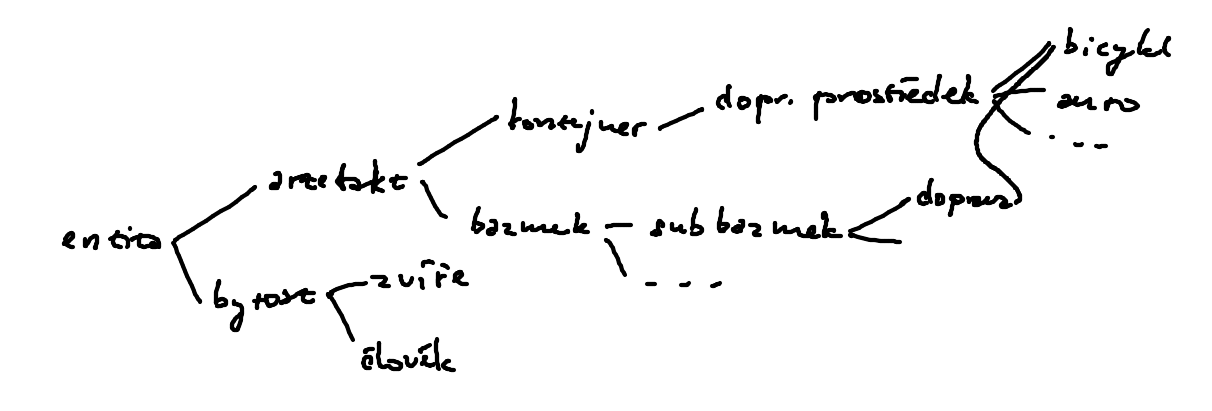
\includegraphics[width=1.0\textwidth]{screenshot_2017-03-31_14-14-36.png}
				% 	\caption{Hierarchizace slovní zásoby ve WordNetu}
				% 	\label{fig:hierchWN}
				% \end{figure}

				% Hierarchická organizace významů substantiv\footnote{a možná i dalších slovních druhů} ve WordNetu tak, jak byla naznačna na grafu \ref{fig:hierchWN} na straně \pageref{fig:hierchWN}, je podpořena i poznatkem, že lidé jsou schopni velice rychle zpracovávat anaforické a kataforické výrazy a komparativní konstrukce. Například ve větě \ex{Vlastnil pušku, ale z té zbraně se nikdy nevystřelilo.} je každému čtenáři zřejmé, že výraz \ex{ta zbraň} odkazuje k výrazu \ex{puška}.\footnote{Zajímavé je uvažovat o významu této věty při vypuštění deiktického \ex{ta} -- zdá se, že pak už anaforický odkaz k \ex{pušce} nefunguje a z věty se stává jakési nesmyslné spojení dvou výroků -- konkrétního (\ex{Vlastnil pušku} a zcela obecného (a evidentně nepravdivého) \ex{ze zbraně se nikdy nevystřelilo}.} Co se zmíněného zpracovávání komparace týče, lze říci, že nelze porovnávat dvě substantiva, která jsou provázána sémantickým vztahem hyperonymie-hyponymie. Výrok \ex{Puška je bezpečnější než zbraň} je zcela nesmyslný. \parencite{pala2013vceska} % nasledujici je asi uplne blbost: \footnote{Porovnání substantiv svázaných vztahem hyperonymie--hyponymie však je možné v případě, že je vypuštěno \ex{než}; specifičtějšímu ze slov se tím pak přisuzuje rys, jenž u hyperonyma není přítomen, či se rys hyperonyma stupňuje: \ex{bytový dům je takový hezčí panelák} či \ex{rys je taková divočejší kočka} (lípa je takový vyšší strom, panelák je takový vyšší dům, ...)}.



			
			% \section{Historie WordNetu}

			% 	- WordNet was created in the Cognitive Science Laboratory of Princeton University under the direction of psychology professor George Armitage Miller starting in 1985
			% 	- been directed in recent years by Christiane Fellbaum
			% 	- George Miller and Christiane Fellbaum were awarded the 2006 Antonio Zampolli Prize
			% 	- As of November 2012 WordNet's latest Online-version is 3.1.

			\section{Sémantické vztahy WordNetu}
			\label{cha:sem-vztahy}

				% Jak bylo naznačeno výše, koncept WordNetu je založen na lexikální sémantice, tedy představě, že slovo je kombinací slovní formy a významu, nebo slovního významu. Slovní forma je projevem \uv{fyzickým}, tedy je to vyřčená či napsaná instance významu. Jak je zjevné z přirozeného jazyka, nelze počítat s tím, že by zobrazení významu na formu bylo bijektivní, tedy každý význam byl namapován jedna ku jedné na slovní formu. V přirozeném jazyce může jedna forma zastupovat více významů a jeden význam může být vyjádřen více formami. Příkladem budiž slovní forma \ex{koruna}, která může zastupovat význam měny, vrcholku stromu, vladařského odznaku, etc. Toto zobrazení jedné formy na více významů se nazývá polysémií nebo homonymií\footnote{obojí znamená totožnost formy pro různé významy, u polysémie však ony významy mají společný základ (byť může být velmi vzdálený)}. S polysémií souvisí ještě homonymie, což ve své podstatě dosti podobný vztah, ale totožnost formy je zcela nahodilá. Kupříkladu formu \ex{kolej} lze interpretovat jako referenci k stopě po voze, případně dvojici kolejnic jako vodící dráze pro dopravní prostředky\td{cit. SSJC} a zároveň jako zařízení vysoké školy pro ubytování studentů.\td{cit SSJC}. U významů formy \ex{koruna} lze vypozorovat nějaký společný základ (koruna stromu je nahoře, panovnickou korunu má panovník na hlavě, tedy nahoře, koruna jako mince zase pravděpodobně získala své pojmenování díky faktu, že na mincích bývá vyobrazen panovník). Naproti obě formy \ex{kolej} pochází z odlišeného základu -- \ex{kolej} jako ubytovací zařízení pochází z latinského \ex{collegium}, kdežto výraz pro dráhu je odvozeno od českého \ex{kolo}\td{cit: etymolog. slovnik, ale jeho online verze to neuvadi}.

				% \textcite{miller1990introduction} popisují výše naznačené vztahy pomocí takzvané lexikální matice. Ta názorně zobrazuje formy synonymní ($F_1$ a $F_2$) a formy polysémní ($F_2$):

				% {\tt tabulka z miller1990introduction pg. 4: http://i.imgur.com/sohtwe5.png}

				% \td{tady by jeste slo pokracovat opisovanim dalsi casti toho clanku (miller1990introduction" pg 5 >>)}

				% V dalších podkapitolách budou rozebrány podrobněji, nikoliv však vyčerpávajícím způsobem, sémentické vztahy konstituující Wordnet. Jelikož se sémantické vztahy pro jednotlivé slovní druhy liší, bude tato kapitola strukturována primárně právě podle slovních druhů a až sekundárně podle sémantických vztahů.

				% proc musi sem. vztahy byt rozdelene podle PoS: o subst. nelze moc rikat, ze jsou antonymni, etc.., 

				% \subsection{Frekvenční distribuce sémantických vztahů ve WordNetu}

					% nejdriv nutno zjistit, jak je to s temi vztahy ruznych slovnich druhu... jinak ta statistika nedava vuebc smysl 

				V této kapitole budou podrobněji rozebrány sémantické vztahy konstituující WordNet. Sémantické vztahy jsou, na rozdíl od vztahů lexikálních, které jsou vztahy mezi slovními formami, vztahy mezi koncepty (významy). Rozdíl nejlépe ilustruje protipříklad. Synonymie je typickým vztahem lexikálním; kdyby byla vztahem sémantickým, znamenalo by to, že dva různé významy (koncepty) mají stejný význam, což je nesmysl, jelikož v tom případě to nejsou dva významy, ale jeden. 

				Struktura těchto vztahů není, jak by se na první pohled mohlo zdát, plochá, ale organizovaná podle syntaktické kategorie významů, jež jsou jimi propojeny. Substantiva mají své vlastní vztahy, stejně tak adjektiva, verba a adverbia. Pojmenování těchto vztahů vychází z lingvistických termínu k nim relevantních (např. \ex{hyperonymie}) a v některých pojmenování některých se napříč různými syntaktickými kategoriemi překrývá, ačkoliv jde o vztahy různé. Například angl. sloveso \ex{run}\footnote{čes. \ex{běžet}} má ve WordNetu jako \ex{hyperonymum} uveden synset s významem \ex{pohybovat se velmi rychle} obsahující slovesa \ex{travel rapidly, speed, hurry, zip}\footnote{čes. \ex{cestovat rychle, uhánět, ...}}. Je evidentní, že tento vztah hyperonymie není identický se vztahem hyperonymie u substantiv, kde \ex{house}\footnote{čes. \ex{dům}} má jako přímé hyperonymum uveden synset \ex{building, edifice}\footnote{čes. \ex{stavba}}. Z činnosti \ex{běžet} vyplývá činnost \ex{rychle se pohybovat}, ale \ex{budova} je pro \ex{dům} nadřazenou třídou. Jde tedy o vztah nikoliv nepodobný, ale ne identický. \td{cit wordnet 3.1 a mozna jeste neco...}

				% Tato kapitola tedy bude primárně organizována podle slovních druhů a sekundárně podle jednotlivých sémantických vztahů.

				
				\subsection{Hyperonymie a hyponymie}

					Vztah nadřazenosti a podřazenosti strukturuje především slovní zásobu substantiv. Hyperonymie je vztahem třídy k podtřídě, hyponymie vztahem podtřídy k třídě. Jde o vztah transitivní a asymetrický. \parencite{miller1990introduction} Díky této hierarchizaci se lze například vyhnout redundanci ukládání informací v paměti, jelikož příznaky třídy není nutné ukládat u každé podtřídy. Podtřída dědí všechny příznaky své mateřské třídy a přidává minimálně jeden další. Například \ex{tramvaj} je \ex{pouličním kolovým přepravníkem, který jezdí po kolejích a je poháněn elektřinou}\footnote{a wheeled vehicle that runs on rails and is propelled by electricity}. Pokud některý ze zděděných příznaků pro podtřídu neplatí, je tento fakt u ní explicitně uložen (podrobněji v kapitole \ref{cha:psycho} na straně \pageref{cha:psycho}). System, v němž jsou atributy takto děděny se nazývá dědičný systém\footnote{inheritance system} (Touretzky, 1986 - The mathematics of inheritance systems\td{dohledat actual knizku}).

					Substantiva jsou ve Wordnetu organizována tak, že každý význam má svůj mateřský význam (hyperonymum), kromě jednoho jediného, a tím je \ex{entity}, tedy uměle vytvořený pojem sloužící jako kořen celé sítě. Jeden koncept může mít hyperonymních významů více, například \ex{house} má jako svá hyperonyma uvedeny synsety \ex{(n) dwelling, home, domicile, abode, habitation, dwelling house} a \ex{(n) building, edifice}. Tato vlastnost mimochodem z WordNetu činí nikoliv stromovou strukturu, jak bývá často vizualizován, ale cyklický graf.\td{src: http://www.randomhacks.net/2009/12/29/visualizing-wordnet-relationships-as-graphs/ a cit neco verohodnejsiho, ale rozhodne bychom mohli namalovat s tim skriptem nejake pekne obrazky..btw, je to cyklicky, ze jo?}

				\subsection{Meronymie a holonymie}

					Meronymie (a k ní komplementární vztah holonymie) jsou, navzdory nepříliš rozšířenému názvosloví, dalším vztahem, jenž je pro uživatele jazyka intuitivní a známý. Jde o vztah \textit{být částí}, potažmo \textit{mít část}. Meronymie je definována tak, že A je meronymem B, pokud A je částí B. Meronymie je vztahem stejně jako hyperonymie transitivním a asymetrickým.\parencite{cruse1986lexical}\td{cit Cruse, 1986, ale vubec tomu nerozumim... http://i.imgur.com/h6NcRVJ.png} Tento vztah také hierarchizuje lexikum do určitých úrovní, ale na rozdíl od vztahu nadřazenosti, v nemž obvykle jeden význam mívá jeden až dva nadřazené významy, u vztahu části a celku by byla situace složitější. Je totiž na snadě, že jeden význam může být meronymem mnoha holonymům -- kupříkladu \ex{dveře} jsou meronymem u \ex{dům}, \ex{auto}, \ex{šatník}, občas \ex{počítačová skříň}, etc. 

					Vztah části a celku je vlastní výhradně substantivům.

				% jeste slovesa - entailment a cause (buy:pay, kill:die)


			\section{Lexikální vztahy ve Wordnetu}

				\subsection{Synonymie}
				\label{cha:synon}

					Synonymie je základním definičním vztahem pro synsety ve WordNetu. Na praktických aplikacích je tento jev nejlépe pozorovatelný, jelikož při vyhledání konkrétní formy je uživateli obvykle nabídnut výběr z jednotlivých významů dané formy. Aby byly od sebe významy oné formy odlišitelné, nabídka běžně se obvykle sestává ze seznamu skupin slovních forem náležejících do nalezených synsetů\footnote{\url{https://www.englishforums.com/English/AdjectiveSatellite/nwzhv/post.htm#1126701}} Kupříkladu při vyhledání slova \ex{kolo} v českém wordnetu tak je uživatel konfrontován s několika skupinami, které obsahují zhruba následující:

					\begin{itemize}
						\item \ex{kolo (1)},
						\item \ex{jízdní kolo (1), bicykl (1), kolo (2)},
						\item \ex{kružnice (1), cívka (1), kolo (3)},
					\end{itemize}

					přičemž čísla (zde) v závorce značí index významu dané formy v daném synsetu. Reprezentace v různých aplikacích a různých wordnetech se liší (standardem bývá číslo významu psát za dvojtečku), koncept však zůstává neměnný. 

					Navzdory zdánilivé jednoduchosti uvedeného konceptu je všeobecnou otázkou, jak synonymii pojímat. Striktní teorie (obvykle připisovaná Leibnizovi) praví, že dvě slova jsou synonymní, pokud se jejich záměnou nikdy nezmění pravdivostní hodnota výroku. Lingvistickou interpretací tohoto poněkud matematicko-logického výroku může pak být, že synonymní dvě slova jsou v případě, že se jejich záměnou nikdy neporuší význam (zhruba ona pravdivostní hodnota) a gramatičnost výroku. Je nasnadě, že takto striktně synonymní slova budou pospolu v jazyce těžko přežívat, jelikož je dokázáno, že jazyk tíhne k ekonomičnosti, která by takovým soužitím dvou slov byla hrubě porušena\td{nejakou citaci na ekonomii jazyka...}. Pravděpodobně jedinými obecně uznávanými synonymy jsou obvykle dvojice cizího slova a domácího slova, například \ex{internacionální} a \ex{mezinárodní}. Jejich záměnou se velice pravděpodobně nikdy pravdivostní hodnota výroku nezmění, stejně tak jako jeho gramatičnost. Stále však zůstává ve hře stylistika, která může být podobnou náhradou narušena (např. z důvodu cílové skupiny čtenářů či stylistické příznakovosti jednoho ze slov (cf. \ex{zajímavý} a \ex{interesantní})). Co se tendence k ekonomičnosti jazyka týče, lze předpokládat, že v těchto případech převládá potřeba synonym k eliminaci opakování určitých slov v textu a tím zajištění jeho stylistické uhlazenosti. 

					Volnější interpretace synonymie počítá ještě s kontextem. Dvě slova jsou synonymní, jsou-li bez způsobení škod nahraditelná alespoň ve stejném kontextu. Jako příklad mohou posloužit formy \ex{board} a \ex{plank}\td{najit ceske priklady}. V kontextu dřevařství mohou tyto dvě formy pravděpodobně bez problému být nahrazeny jedna za druhou, ovšem v případě, že je forma \ex{board} použita ve významu \ex{comittee}, těžko ji lze nahradit formou \ex{plank}, neboť by se věta obsahující takové nahrazení stala zcela nesmyslnou.

					Bylo by nanejvýš logické považovat synonymii za vztah diskrétní, tedy že dvě formy buďto synonymní jsou, či nejsou. Z logického hlediska to nepochybně z již uvedeného vyplývá, ovšem lingvisticko-filosofický náhled výcházející z poznatků reálného jazyka na tuto problematiku nahlíží poněkud odlišně. Synonymie v striktním slova smyslu je velice vzácná. Její volnější interpretace je značně častější, ale také výrazně vágnější -- kontext, v němž dvě formy synonymní jsou, může být velmi široký, či naopak velice úzký. Záměna některých dvojic (či spíše obecně n-tic, volné synonymní řady mohou být vcelku dlouhé -- \ex{textil:1, látka:1, textilie:2, plena:1, tkanina:1}\td{cit. cesky WN}) může měnit stylistiku a význam výpovědi více či méně, přičemž ony dvě formy stále dle daných kritérií lze považovat za synonymní. Nelze tedy než vyvodit, že synonymie, minimálně z pohledu přirozeného jazyka, je jevem graduálním, a některé formy jsou tak \textit{synonymnější} než jiné. \parencite{miller1990introduction}

					Zaměnitelnost forem podporuje ještě jeden koncept, na němž je WordNet postaven, a to fakt, že jednotlivé významy jsou seskupovány podle slovních druhů. Tento systém vede k jisté redundantnosti, jelikož zvláště v syntetických\td{check, nekecam?} jazycích, jako je kupříkladu angličtina, lze nalézt mnoho případů, kdy identická slovní forma zastupuje více slovních druhů. Významy, které taková slovní forma zastupuje (napříč slovními druhy), mohou být velice blízké, nikdy však nebudou stejné (nelze říci, že význam slovesa \ex{run}\footnote{běžet} a substantiva \ex{run}\footnote{běh} je identický). Jejich záměnou by se sice nestalo vůbec nic, jelikož čtenář či posluchač textu, v němž taková záměna nastala, by automaticky formu interpretoval ve prospěch správného slovního druhu, avšak pokud by slovní druh byl nějakým způsobem \uv{vynucen} (nechť nyní čtenář pomine úvahy, jakým způsobem lze \textit{vynutit} slovní druh formy), stala by se výpověď zcela negramatickou a nesmyslnou. 

					Jakkoliv to není přímo svázané se synonymií, je na místě\td{ne, neni, ale nechtelo se mi mazat 2k napsanych znaku xD} poznámka o výskytu stejné formy v různých synstetech. Slovo je kombinací slovní formy a významu, nebo slovního významu. Slovní forma je projevem \uv{fyzickým}, tedy je to vyřčená či napsaná instance významu. Jak je zjevné z přirozeného jazyka, nelze počítat s tím, že by zobrazení významu na formu bylo bijektivní, tedy každý význam byl namapován jedna ku jedné na slovní formu. V přirozeném jazyce může jedna forma zastupovat více významů a jeden význam může být vyjádřen více formami. Příkladem budiž slovní forma \ex{koruna}, která může zastupovat význam měny, vrcholku stromu, vladařského odznaku, etc. Toto zobrazení jedné formy na více významů se nazývá polysémií nebo homonymií\footnote{obojí znamená totožnost formy pro různé významy, u polysémie však ony významy mají společný základ (byť může být velmi vzdálený)}. S polysémií souvisí ještě homonymie, což ve své podstatě dosti podobný vztah, ale totožnost formy je zcela nahodilá. Kupříkladu formu \ex{kolej} lze interpretovat jako referenci k stopě po voze, případně dvojici kolejnic jako vodící dráze pro dopravní prostředky\td{cit. SSJC} a zároveň jako zařízení vysoké školy pro ubytování studentů.\td{cit SSJC}. U významů formy \ex{koruna} lze vypozorovat nějaký společný základ (koruna stromu je nahoře, panovnickou korunu má panovník na hlavě, tedy nahoře, koruna jako mince zase pravděpodobně získala své pojmenování díky faktu, že na mincích bývá vyobrazen panovník). Naproti obě formy \ex{kolej} pochází z odlišeného základu -- \ex{kolej} jako ubytovací zařízení pochází z latinského \ex{collegium}, kdežto výraz pro dráhu je odvozeno od českého \ex{kolo}\td{cit: etymolog. slovnik, ale jeho online verze to neuvadi}.

					Seskupování významů podle slovních druhů a seskupování forem dle vztahu synonymie se tedy zdá v případě lexikální databáze určené pro strojové zpracování jako vhodným konceptem. Oproti tradičním slovníkům se totiž počítačově zpracovávaná lexikální databáze nemusí potýkat s problémem lidského faktoru -- jednotlivé synonymické řady je stroj schopen prohledávat, na rozdíl od člověka, velice účině, a nahradí tak v případě, že WordNet používá člověk, neúčinné lidské procházení restříkového obsahu.\td{psano v chvatu, mohlo by se to mozna trochu uhladit...}

					% centralni jednotka WN, davalo by smysl rozlisovat syn. mezi formami a mezi vyznamy, ale pro technickou jednoduchost se to nedela; je to symetricka relace a pokud jsou ji spojeny vyznamy, pak i jejich formy; zamenitelnost - silna: zamenou se nemeni pravdivost vyroku, slabsi: podle kontextu - vyznam se v kontextu zamenou nezmeni (plank × board); z toho plyne nutnost redundance slovnich druhu (show a show nelze zamenit); z log. hlediska diskretni (bud slova syn. jsou ci ne), ale z lingv./fil. hlediska gradient - nektere dvojice jsou syn~ctejsi nez jine- porad je to ale reflexivni; 
					
				% slovesa nemaji meronymii, ale has_a relation -- entailment

				\subsection{Antonymie}
					% problem s terminologii -- co jeste je antonymum, a co uz ne (muz-zena?)
					% pouziti ve slovnicich velmi siroke
					% stupnovatelnost, neutralni prostor na skale, vs. nestupnovatelna adj. - komplementarni, X entails not Y, vs. red-green
					% miller1990introduction tvrdi, ze to neni semanticky, ale lexikalni vztah

					Antonymie, neboli protiklad, je navzdory zdánlivé triviálnosti koncept překvapivě těžce definovatelný. Všeobecně se antonymií rozumí významová opozice, faktem však je, že použití tohoto termínu je velmi široké a druhů antonymie je několik. Nejjednodušším druhem je například antonymie mezi adjektivy \ex{živý} a \ex{mrtvý}. Negace prvého automaticky značí druhé a naopak (je-li řeč o živých bytostech), jelikož v reálném světě neexistuje žádný další třetí stav. Tento jednoduchý vztah však nefunguje vždy -- například s adjektivy \ex{bohatý} a \ex{chudý} je to jiné. Mnoho lidí se nepovažuje ani za chudé, ani za bohaté, a tudíž z toho, že někdo není bohatý, automaticky neplyne to, že by byl chudý. \textcite{miller1990introduction} Zajímavé je, že tento vztah není reflexivní. Pokud někdo není bohatý, tak to nemusí znamenat, že je chudý, ale pokud je o někom tvrzeno, že \textit{je} bohatý, tak to nutně znamená, že \textit{není} chudý. \textcite{paradis2006antonymy} 

					Rozdíl mezi výše uvedenými dvojicemi, tedy \ex{mrtvý:živý} a \ex{chudý:bohatý} spočívá ve stupňovatelnosti daných adjektiv. Pro ilustraci -- lze říci, že někdo je \ex{bohatší} než někdo jiný, ale nelze říci, že někdo je \ex{\textit{mrtvější}} než někdo jiný. Pokud jsou adjektiva stupňovatelná, tedy lze říci, že objekt A je více X než objekt B, neoznačují komplementární stav, ale graduální vlastnost. Označované pak může být zařazeno kamkoliv mezi tyto dva póly, přičemž nachází-li se v pomyslné střední šedé zóně, nelze jej označit výrazy odpovídajícími pólům gradientu. Tvrzení, že někdo \ex{není ani chudý, ani bohatý}, dává smysl, protože tato adjektiva označují extrémní stavy, mezi nimiž je prostor pro normální stav. \textcite{paradis2006antonymy} 

					Vztah antonymie ve WordNetu je koncipován tak, aby zřejmě byl co nejpodobnější uvažování široké populace uživatelů jazyka, tedy užívá primitivního konceptu antonymie. Některé studie dokonce za antonymní považují výrazy pouze vágně, intuitivně protikladné, jako například \ex{muž:žena} či \ex{chytrý:hloupý}. \parencite{lehrer1982antonymy}

					% taky dopsat neco o tom, ze antonyma jsou si zaroven nejblizsi a zaroven nejvzdalenejsi (lisi se jednim priznakem a jsou na opacnych polech) -- paradis2006antonymy

					% Antonymie podle \textit{miller1990introduction} navíc ani není sémantickým vztahem, ale lexikálním, .. a tuhle poznamku bych si nechal na konec, jelikoz to celkem zabiji.

					Ve WordNetu se antonymie vyskytuje u substantiv (\ex{man:woman}), adjektiv (\ex{rich:poor}, a dokonce i \ex{white:black} v rasovém významu\footnote{cf. také antonymní vztah \ex{Caucassian:black} ve WN}), verb (\ex{open:close}) i adverbií (\ex{well:ill}).


					% tak jaky tam vlastne jsou vztahy? jsou deleny pro PoS, ci nikoliv?
		% chapter princeton_wn (end)

		\chapter{Další wordnety}
		\label{cha:dalsi_wordnety}

			% base concept 
				% - koncept, kterej je co nejvys v sem. hierarchii a ma spoustu vztahu na dalsi koncepty (ale proc?)
				% - universalita: 
		
			Podle vzoru princetonského WordNetu začaly postupně vznikat i další sémantické sítě založené na stejném konceptu. Tyto sémantické sítě se samozřejmě svou strukturou do větší či menší míry liší\td{nakou kurva citaci}, hlavním kritériem pro to, aby mohly být považovány za wordnet, je to, aby obsahovaly synsety a hyponyma. \parencite{gwa2013wordnetsworld} % Jelikož se tato práce bude primárně zabývat wordnetem českým, bude pro srovnání uvádět dva hlavní evropské vícejazyčené wordnety, a to Eurowordnet a Balkanet. 

			\section{EuroWordNet} % (fold)
			\label{sec:eurowordnet}
				
				% motivace - aby bylo mozny delat nfo retrieval, search queries augment
				% prolinkovani s PWN1.5 pomoci ILI - interlingual index
					% plochy, aby nereflektoval organizaci nejakeho konkretniho WN
				% odlisne vztahy od PWN

				EuroWordNet je mezinárodní lexikální databáze pro osm evropských jazyků (angličtina, čeština, dánština, francouzština, italština, němčina, španělština). Jde o soubor jednotlivých národních wordnetů, které jsou propojeny takzvaným mezijazykovým indexem (ILI, \textit{inter-lingual-index}). Obecně jsou wordnety Eurowordnetu založené svou strukturou na princetonském WordNetu (verze 1.5), ale z důvodu různorodosti jazyků se v některých aspektech od něj odlišují.

				Základní motivací pro vznik EuroWordNetu byla evropská jazyková různorodost a z ní pramenící problémy ve zpracování dat a napomáhání uživateli v přístupu k neanglickým datům. Vossel 1999 (Vossen-Eurowordnet.pdf, pg XX) argumentuje, že uživatel musí umět anglicky a být obeznámen s tím, jak je zdroj, v němž vyhledává napsán, aby byl schopen v něm účinně hledat. Vytvořením wordnetů pro jiné jazyky si slibuje, že se zlepší možnost přístupu uživatelů k neanglickým datům, možnosti inference znalostí z těchto dat a případně i mezijazykové vyhledávání. Poslední je založeno na faktu, že od počátku byly jednotlivé wordnety EuroWordNetu vytvářeny s tím, že budou propojeny na základě základních konceptů (BCS, \textit{Base Concepts}\td{rikam to dobre? vubec jim nerozumim}) a mezijazykového indexu.

				Jelikož se jednotlivé jazyky zapojené v projektu EuroWordNetu značně odlišují ve struktuře své slovní zásoby, jsou jednotlivé wordnety nezávislé. To znamená, že se mohou odlišovat například svou hierarchizací. Stejný koncept tak může ve dvou různých wordnetech mít různá hyperonyma, meronyma, etc., protože například anglické označení pro prst je odlišené, pokud jde o prst na noze (\ex{toe}), či na ruce (\ex{finger}). Podobně má v jiném příkladu dánština odlišené označení hlavy u zvířat vyjma koní, tedy \ex{kof}, a hlavy lidské a koňské (\ex{hoofd})\td{nekde jsem to cetl, ale nemuzu to dohledat (a slovnik to popira, tak to mozna bude jiny jazyk... dunno, TB fixed}. \parencite{vossen1997eurowordnet}

				Národní wordnety jsou vzájemně propojené přes mezijazykový index s anglickým wordnetem, který je obsahově založený na princetonském WordNetu, ale není identický. Anglický wordnet byl přizpůsoben strukturně tak, aby byl použitelný v EuroWordNetu, tedy byly přidány dodatečné metainformace a druhy vztahů (podrobněji dále). V národních wordnetech existuje několik druhů konceptů, které jsou rozlišeny podle příbuznosti s koncepty v ostatních národních wordnetech. Pokud je koncept přítomen ve všech wordnetech EuroWordNetu, jde o koncept tzv. \textit{Global Base Concept} (GBC). Koncept, jenž jen přítomen v alespoň dvou národních wordnetech je označován jako \textit{Common Base Concept} (CBC) a v poslední řadě koncept, který se vyskytuje pouze v jednom národním wordnetu nese označení \textit{Local Base Concept} (LBC). \parencite{gwa2013baseconcepts} Propojení konceptů společných pro více jazyků je zajištěno pomocí jednotných identifikátorů a mezijazykového indexu, který je nadmnožinou všech konceptů v EuroWordNetu. ILI je hierarchicky plochá struktura (proto \textit{index}, nejde o další \uv{všejazykový} wordnet). \parencite{vossen1997eurowordnet}

				Jelikož v době, kdy EuroWordNetu vznikal, byl princetonský WordNet poněkud omezený mimo jiné co se vztahů mezi slovními druhy týče, vznikly pro EuroWordNet speciální vztahy umožňující úplnější práci s významy. Základní vztahy přejaté z princetonského WordNetu 1.5 jsou uvedeny v tabulce \ref{wn-rels} na straně \pageref{wn-rels}.

				\begin{table}[t]
					\centering
					\label{wn-rels}
					\begin{tabular}{l l l}
					Relace                           & Slovnědruhové kombinace & Příklad                \\\hline
					antonymie                        & A-A, V-V                & open:close             \\\hline
					hyponymie                        & N-N, V-V                & car:vehicle, walk:move \\\hline
					meronymie                        & N-N                     & head:nose              \\\hline
					vyplývání\footnote{entailment} & V-V                     & buy:pay                \\\hline
					následek                         & V-V                     & kill:die               
					\end{tabular}
					\caption{Vztahy přejaté z princetonského WN (N: substantivum, A: adjektivum, V: verbum)}
				\end{table}

				Navíc k těmto vztahům byly přidány štítky (\textit{labels}), jež relaci konkretizují. Byly použity následující štítky:\td{nikdy jsem to nevidel, pls je to nekde v nasich WN na debdictu?}

				\begin{itemize}
					\item conjunction/disjunction
					\item non-factive
					\item reversed
					\item negation
				\end{itemize}

				Použití konjunktivního a disjunktivního štítku spočívá v myšlence, že například u meronymie by bylo vhodné rozlišovat, zda jde o části, které dohromady tvoří celek, nebo jde o podčásti částí (např. \ex{nůž} má meronyma \ex{čepel}, \ex{rukojeť}, \ex{ostří}, ale \ex{ostří} je ve skutečnosti meronymem až \ex{rukejeti}, nikoliv přímo samotného \ex{nože}\td{vubec netusim, jestli to chapu spravne, spis mi prijde, ze ne..}).

				Štítek \textit{non-factive}\td{jak to prelozit? nezda se mi, ze by to melo s timhle cokoliv spolecneho: https://goo.gl/7Zw1SG} je používán u kauzální relace, která nemusí být nutně naplněna:

					% \begin{itemize}
					% 	\item \ex{zabít}\hskip 3em \textit{vyústí v}\hskip 3em \ex{zemřít}
					% 	\item \ex{hledat}\hskip 3em \textit{vyústí v}\hskip 3em \ex{najít} \texttt{non-factive}
					% \end{itemize}

					\begin{table}[h]
					\centering
					% \caption{My caption}
					\label{my-label}
					\begin{tabular}{lllcc}
						příčina	& vztah & následek & non-factive? & nutně vyplývá? \\ \hline
						\ex{zabít}  & \textit{vyústí v} & \ex{zemřít} & – & ano                       \\
						\ex{hledat} & \textit{vyústí v} & \ex{najít} & \texttt{non-factive} & ne
					\end{tabular}
					\end{table}

				Podobně lze upřesnit pomocí štítků další relace tak, že jsou ve výsledku jednoznačnější a wordnet, v němž jsou takto označené vztahy obsaženy, může poskytovat více informací. 

				% prostor pro rozsireni

				Jako další vylepšení oproti tehdejší verzi princetonského WordNetu přinesl EuroWordNet také relace mezi slovními druhy a vztah blízkého synonyma\td{hmm, a co near antonym? to be investigated}. Argument pro zavedení mezislovnědruhových relací je relativně přímočarý, a to, že umožňují \uv{sblížit} koncepty, které jsou si příbuzné, jen náleží k jinému slovnímu druhu. Nutno podotknout, že v době vzniku této práce je princetonský WordNet ve verzi 3.1 a obsahuje už relaci \ex{derivationally related form}, která zajišťuje přesně toto propojení (více o synsetech v princetonském WordNetu v kapitole \ref{cha:princeton-synset-rels} na straně \pageref{cha:princeton-synset-rels}). Co se vztahu blízkého synonyma (\ex{near synonym}) týče, důvodem pro jeho zavedení byl údajně zájem mít možnost přiblížit koncepty, které jsou si významově podobné, ale pouze na své úrovni. U takových konceptů platí, že byť jejich význam je podobný, jejich hyponyma nelze zařadit pod jeden koncept, jelikož se rozdíl mezi oněmi koncepty svázanými vztahem blízkého synonyma prohlubuje. Příkladem budiž trojice nizozemských slov \ex{aparaat}, \ex{werktuig} a \ex{instrument}, jež jsou si významově nepříliš vzdálená:

				% \Tree[.voorwerp\\objekt 
				% 		[.lichaam\\tělo]
				% 		[.aparaat\\přístroj]
				% 		[.werktuig\\nástroj][.instrument\\pomůcka]
				% 	]

				\begin{figure}[h]
					\centering
					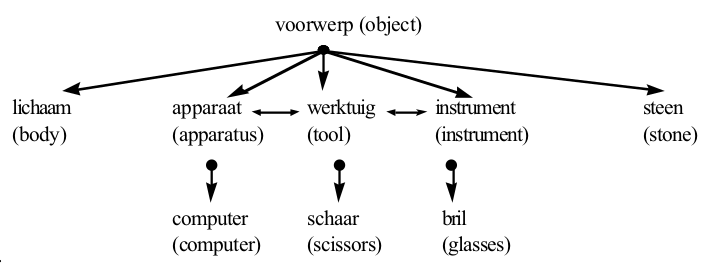
\includegraphics[width=1.0\textwidth]{stromcik-nlNL.png}
					\caption{Blízká synonyma (k překreslení)}
					\label{fig:near-synon}
				\end{figure}

				Jak je z obrázku \ref{fig:near-synon} na straně \pageref{fig:near-synon} zřejmé, všechna hyponyma slova \ex{voorwerp} (\ex{objekt}) jsou si rovna, avšak některá jsou si rovnější\td{smim v diplomce delat reference na kvalitni literaturu? xD}. Tři výše zmíněná slova jsou si navzájem významově výrazně bližší, než jsou si blízká s ostatními hyponymy na jejich úrovni. Právě aby bylo možno tento vztah reflektovat a tím docílit možnosti například nahrazovat za sebe slova, která sice nemohou být ve stejném synsetu, ale jsou si podobná, byl zaveden vztah blízkého synonyma. Lze totiž předpokládat, že uživatel jazyka podobná slova také může zaměnit. \parencite{vossen1997eurowordnet} \td{cela ta kapitola je v podstate z toho vossena, tak nevim, jak to citovat :/}

				% cely Vossen-Eurowordnet.pdf
				
				% neco psat o Balkanetu?

				\section*{poznamky}

				Jak moc mam rozebirat další wordnety (resp. site WN, jako je Eurowordnet, balkanet...)? 

				Jak dal: Dal bych chtel rozebrat nejak obecne vizualizace WN (ze ne vsechno lze nacpat do jedny), jaky se obecne voli pristupy (fuck everything, delame jen hyponymii, vetsinou), a pak vybrat par nejakejch dobre pristupnejch a/nebo originalnich, ktery rozebrat, proc jsou spatny...

				\subsection*{co nechapu:}

				\begin{itemize}
					\item adjektiva (jakysi model s kolem (stred kola nejakej core), sprinclikama k obvodu (vztahy k "satelite adjectives"), osa k dalsimu "stredu kola"... )
					\item nevim, kde najit rozdily mezi Princeton WN verzema (1.5 vs 2.1 vs. 3.0)
				\end{itemize}

	\part{Přehled a porovnání existujících vizualizací sémantických sítí}

		Tato část textu bude zaměřena na zmapování existujících dostupných rozhraní a jejich zhodnocení. Výčet jednotlivých rozhraní rozhodně není vyčerpávající, jelikož některé vědecké instituce mohou vyvíjet své nástroje pro práci se sémantickými sítěmi neveřejně, některé nástroje už nejsou dostupné, etc. Nástroje pro vizualizaci\footnote{Terminologická poznámka: v této práci je vizualizací dat wordnetů míněna vizualizace jak textová reprezentace, tak grafická.} dat wordnetů byly vybírány pro přehled v této práci podle několika kritérií relevantních především pro koncového uživatele, avšak i pro případné vývojáře dalších wordnetů (tedy zda dané rozhraní mohou použít pro svá data).

		\chapter{Metodologie porovnání}

			\section{Výběr rozhraní}

				Hlavním kritériem pro zařazení do rozhraní do výběru byla jeho dohledatelnost podle vyhledávacího dotazu na indexovací a vyhledávací webové stránce \url{https://www.google.com}. Dotazy byly voleny tak, aby bylo dosaženo co nejvyšší relevance vyhledaných výsledků:

					\begin{itemize}
						\item wordnet visualization
						\item wordnet visualisation
						\item wordnet graph
					\end{itemize}

				% mozna vypsat vysledky a zaradit ten seznam sem? plus nejak exaktneji algoritmus filtrovani?
				Z přehledu byly samozřejmě vyřazeny implementace, které k době hledání\footnote{20. dubna 2017} už nebyly dostupné. Také nebyla zahrnuta rozhraní, která jsou funkčně podobná jiným. Ačkoliv většina existujících rozhraní zřejmě pracuje buďto výhradně s princetonským WordNetem, či jej jako zdroj dat nabízí jako jednu z možností, nebylo na toto bráno ohled. Do přehledu byla zahrnována především rozhraní, která jsou dostupná z webového prohlížeče, jelikož je to pro koncového uživatele nejpohodlnější způsob přístupu k aplikaci (není nucen instalovat žádný přídavný software na svůj počítač), ovšem vzhledem k rozšířenosti rozhraní určených pro aplikační prostředí Java byla do přehledu zahrnuta i některá rozhraní právě tohoto typu. Jsou však popisována pouze povrchněji a měla by při interpretaci hodnocení být automaticky značně penalizována, jelikož je uživatel mající zájem takové rozhraní použít nucen instalovat aplikační rozhraní Java, pokud jej nemá. Dalším důvodem k penalizaci je také fakt, tyto aplikace nejsou přímo spustitelné na mobilních zařízeních\footnote{Pro Android existuje emilační rozhraní XY link, lze však předpokládat, že použitelnost vizualizací wordnetu bude na zařízení s malou obrazovkou poněkud omezená.} \parencite{gronli2014mobile} a jejich portabilita do formy nativních aplikací může omezená a obtížná.

				Podstatná z hlediska hodnocení je také univerzalita, tedy zda je zdrojový kód rozhraní otevřený a je možné jej použít i pro vizualizaci jiné sémantické sítě, než pro kterou bylo rozhraní vyvinuto. Je ovšem dlužno podotknout, že tato informace bývá často nedostupná; potom se v rámci této práce předpokládá, že kód otevřený není.

				Do přehledu byla tedy zahrnuta následující rozhraní:

					\begin{itemize}
						\item An interactive visualization of the Princeton WordNet database (\url{http://mateogianolio.com/wordnet-visualization/})
						\item WordNET Editor (\url{http://wordventure.eti.pg.gda.pl/wne/wne.html})
						\item Cornetto Demo (\url{http://cornetto.clarin.inl.nl/wordnet.xql?ssID=&word_form=&pos=&sense_pos=1})
						\item WordVis (\url{http://wordvis.com/})
						\item sloWTool (\url{http://nl.ijs.si/slowtool/})
						\item BabelNet (\url{http://babelnet.org})
						\item wnbroswer\footnote{sic erat scriptum} (\url{http://homepages.inf.ed.ac.uk/adubey/software/wnbrowser/index.html})
						\item Visual Browser (\url{https://nlp.fi.muni.cz/projekty/visualbrowser/})
						\item Treebolic (\url{})
						\item Artha (\url{http://artha.sourceforge.net/wiki/index.php/Home})
						\item GoldenDict (\url{http://goldendict.org/})
						% \item GRAPH WORDS online thesaurus (\url{http://graphwords.com/})
					\end{itemize}

				Pro účely porovnání (určení východiska\td{well, baseline}) bude do popisu zahrnuto ještě jedno rozhraní, a to oficiální vyhledávací rozhraní princetonského WordNetu (\url{http://wordnetweb.princeton.edu/perl/webwn}). 

			\section{Strukturalizace přehledu a kritéria hodnocení}

				Výše vypsaná rozhraní budou v dalších kapitolách rozdělena podle toho, zda umožňují přístup z webového přihlížeče (nativně, bez nutnosti mít nainstalované prostředí Java\td{nejakej link, mozna vysvetleni?}), budou zhodnoceny jejich positiva a negativa z hlediska použitelnosti pro získání informací o hledaném výrazu a v neposlední řadě také podle toho, jak kvalitní jejich uživatelské rozhraní je. 

				K rozdělení podle dostupnosti bylo přistoupeno jednak proto, že v době vzniku této práce je pokročilost webových technologií dostatečná k tomu, aby podobné vizualizace byly tvořeny jako webové stránky, a jednak proto, že cílem této práce je vytvořit všeobecně dostupné a použitelné rozhraní k wordnetům. Všeobecně použitelným je míněna použitelnost nejen na osobních počítačích, ale také na mobilních zařízeních, což v podstatě vyřazuje použití technologií jako jsou zásuvné moduly Java používané k realizaci různých existujících rozhraním (příkladem budiž \ex{Visual Editor}). 

				Rozhraní jsou hodnocena na základě několika kritérií. Cílem je porovnat jejich přínos v kontextu ostatních existujících rozhraní a v kontextu současných trendů webových aplikací a ilustrovat, s jakými problémy se všeobecně rozhraní potýkají.  Z tohoto důvodu právě nebyla do přehledu zařazována rozhraní, která se podobají svou funkcionalitou a ovládáním rozhraním již zařazeným. Kritéria hodnocení v této práci jsou následující:

					\begin{itemize}
						\item přínos oproti základnímu oficiálnímu rozhraní princetonského WordNetu
							\begin{itemize}
								\item originální vizualizace dat vedoucí k možnosti identifikovat trendy v datech, které zůstávají uživateli skryty případě základní textové reprezentace dat
								\item reprezentace dat vhodnější z hlediska zásad přístupnosti webu\footnote{web accessibility}
							\end{itemize}
						\item responsivita rozhraní -- kvalitní použitelnost rozhraní i na zařízeních s menší obrazovkou, jako jsou mobilní zařízení typu chytrý telefon či tablet
						\item v případě webových aplikací ukládání stavu aplikace v adresním řádku prohlížeče (umožňuje sdílení nebo založení odkazu ke konkrétnímu hledání a zachování nastavení aplikace)
					\end{itemize}

			\section{Podmínky testování}

				Pro testování rozhraní, které bylo pro účely této práce provedeno, byl použit operační systém Ubuntu 16.04 LTS v 64bitové verzi, webový prohlížeč Pale Moon ve verzi 27.1.1 (rovněž 64bitový) s nastavaným uživatelským agentem na Firefox (z důvodů kompatibility). Ačkoliv se počítalo, vzhledem k nepříliš rozšířenému vykresovacímu jádru toho prohlížeče, s možnými problémy v zobrazení některých rozhraní, nebyly tyto zjištěny, a tak nebylo nutné provádět testování rozhraní ještě v dalších prohlížečích. Lze předpokládat, že v rozšířených prohlížečích, jako jsou Firefox či Chrome, budou jednotlivá rozhraní fungovat a vypada podobně, jako v prohlížeči Pale Moon.

				Testování na mobilním chytrém telefonu bylo prováděno na zařízení Nexus 5 (displej s úhlopříčkou 5" a rozlišením 1080 × 1920 px) s operačním systémem Android 6 v prohlížeči Chrome (sestavení 57.0). Možnost \textit{request desktop site} byla nastavena na \textit{vypnuto}.

			\section{WordNet Search jako základ porovnání}
			\label{wnvis:wnsearch}

				Oficiální rozhraní k princetonskému WordNetu je koncipováno jako textová reprezentace dat, přičemž, byť volitelně, umožňuje zobrazovat veškeré k hledanému výrazu relevantní informace, jež WordNet obsahuje. Data jsou vizualizována jako soubor seznamů.

				Po vyhledání zadaného výrazu jsou uživateli prezentovány v bodech jednotlivé synsety obsahující hledanou slovní formu rozdělené podle slovních druhů, k nimž přináležejí. V základním nastavení každý bod sestává ze slovních forem tvořících daný synset, jeho definici, případný příklad užití a odkaz na detaily synsetu. Kliknutím na tento odkaz se zobrazí v podseznamu sémantické a lexikální relace, v nichž je daný synset přítomen. Samotné relace jsou opět odkazy, jejichž otevřením je uživateli prezentován seznam synsetů, které jsou spolu s daným synsetem v dané relaci přítomny. Postupným otevíráním detailů synsetů v podseznamech se lze zanořovat hlouběji a hlouběji do struktury, resp. se ve struktuře vzdalovat původnímu synsetu po hranách relací.

				Uživatel má možnosti si zvolit množství informací, jež jsou mu prezentovány, a to od úplného minima (pouze slovní formy nalezených synsetů a jejich syntaktické kategorie) až po vše, co se ve WordNetu vyskytuje, včetně identifikátorů a dalších technických detailů. Rozhraní svůj stav ukládá jako parametry URL\footnote{Uniform Resource Locator}, takže je možné jej pozdějí obnovit z adresy.

				Rozhraní není responsivní, ale vzhledem k tomu, že je v základu relativně úzké (pod 700 px), je na chytrém telefonu použitelné.

				\begin{figure}[h]
					\centering
					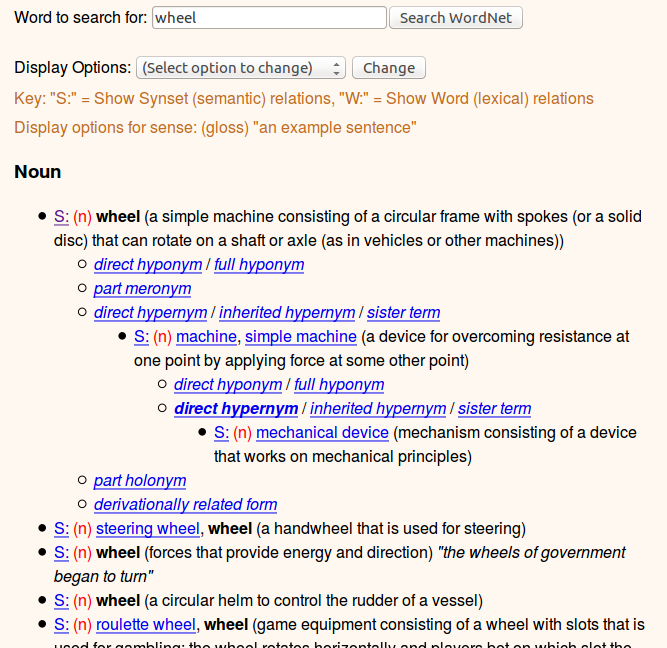
\includegraphics[width=1.0\textwidth]{wnsearch.png}
					\caption{Ukázka rozhraní: WordNet Search 3.1 v základním nastavení a s otevřenými detaily synsetů}
					\label{fig:wnsearch}
				\end{figure}

				Podobnou jako WordNet Search splňují i některá další rozhraní. Za zmínku stojí například WNSearch\footnote{\url{http://www.golovchenko.org/cgi-bin/wnsearch}}, což je minimalistické čiště textové rozhraní, které díky absenci jakýchkoliv stylů je responsivní a dobře použitelné na mobilních zařízeních s libovolně velkým displeje. Mezi další rozhraní s podobnou funkcionalitou patří URCS Wordnet Browser (pro Javu)\footnote{\url{http://www.cs.rochester.edu/research/cisd/wordnet/}} či GoldenDict (rozhraní pro stolní počítače\footnote{myšleno všeobecně pro zařízení typu stolních počítačů, laptopů, případně tabletů etc., na nichž je provozován operační systém nikoliv určený pro mobilní zařízení})\footnote{\url{http://goldendict.org/}}.

		\chapter{Vizualizace s webovým rozhraním}

			Jako bylo naznačeno v úvodu této části, vizualizací s webovým rozhraním se v této práci míní taková implementace, která ze strany uživatele nevyžaduje instalaci žádných doplňujících aplikací či aplikačních prostředí\td{lze takhle nazvat Javu?} kromě samotného webového prohlížeče.

			\section{An interactive visualization of the Princeton WordNet database}
			\label{wnvis:intviswn}

				Jeden z projektů programátora jménem Mateo Gianolio z Lundské univerzity (Švédsko)\td{src: https://www.linkedin.com/in/mateo-gianolio-a89558b6/?trk=profile-badge-name}. Jde o jednoduché rozhraní napojené na princetonský WordNet, které po zadání hledaného výrazu zobrazí synsety obsahující daný výraz. Jednotlivé synsety jsou barevně odlišeny podle syntaktických kategorií (slovních druhů), k nimž náležejí, a uspořádány kruhově kolem hledaného výrazu. Z každého synsetu je vždy zobrazena jen první slovní forma. Pokud uživatel najede kursorem myši na některý ze synsetů, zobrazí se další případné slovní formy náležející do daného synsetu a jeho glosa (definice), je-li dostupná.

				Další slovní formy v nalezených synsetech jsou klikatelné, což umožňuje dostat se přes ně na synsety obsahující onu slovní formu, na níž bylo uživatelem kliknuto (s identickým výsledkem, jako kdyby dané slovo uživatel zadal do vyhledávacího pole).

				Ačkoliv úvodní odstavec na stránce s rozhraním vybízí uživatele k \uv{prozkoumání desambiguace slov}\td{cit web}, zobrazují výsledky hledání pouze synsety a slovní formy do nich náležející, přičemž synsety připojené sémantickými vztahy hyponymie, meronymie etc. nejsou zobrazitelné (jinak než případným náhodným výskytem jedné slovní formy ve více synsetech). To použití WordNetu omezuje na obyčejný thesaurus.

				Samotný design grafického rozhraní je řešen poněkud nešťastně a působí dojmem, že cílem autora bylo prokázat své schopnosti používat různé standardní tranformační funkce CSS.\td{odkazat na kapitolu o CSS nekde dal a mozna to, ze to je fakt v CSS...} Pro indikaci běžícího procesu vyhledávání byl použit efekt rotační animace pro vyhledávací pole a po dokončení vyhledávání jsou výsledky zobrazeny paprskovitě okolo vyhledávacího pole. To způsobuje, že některé texty jsou zobrazeny pod úhlem až 90 stupňů, což může pro některé uživatele činit jejich přečtení obtížnějším. 

				Rozhraní není tzv. responsivní, tedy nepřizpůsobuje se velikosti obrazovky, na níž je zobrazeno. 

				Toto rozhraní tedy poskytuje velice omezený přístup k datům WordNetu a neposktuje žádné výhody oproti základnímu oficiálnímu rozhraní k princetonskému WordNetu. Jeho grafické pojetí je čistě arbitrární, neslouží žádnému účelu a naopak zhoršuje jeho použitelnost.

				\begin{figure}[h]
					\centering
					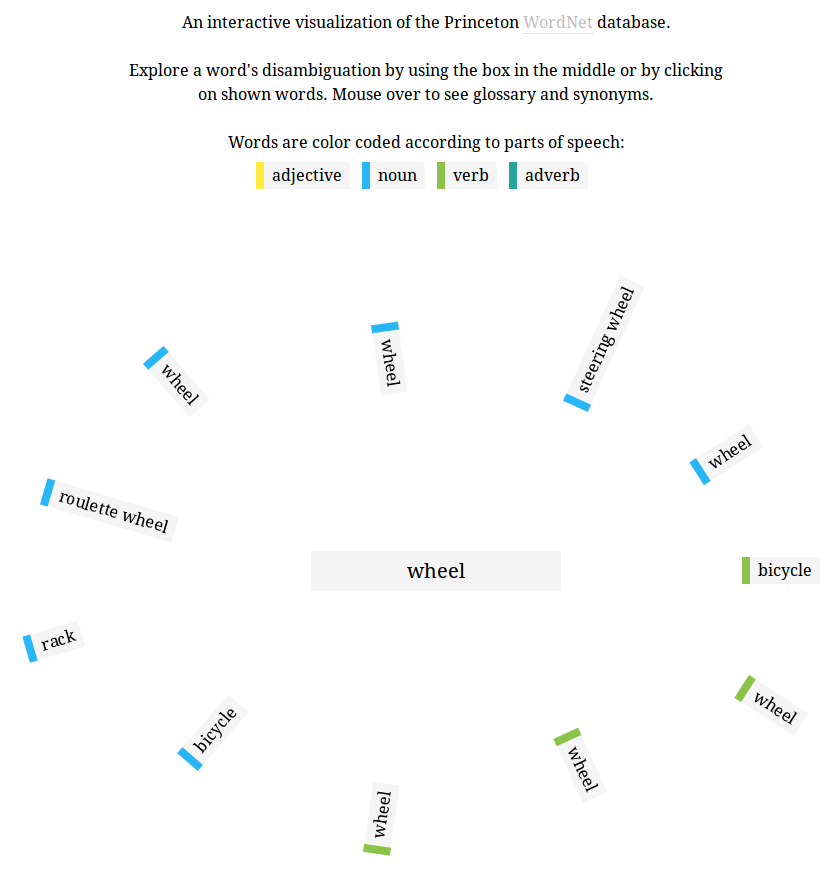
\includegraphics[width=0.8\textwidth]{intviswn.png}
					\caption{Ukázka rozhraní An interactive visualization of the Princeton WordNet database}
					\label{fig:intviswn}
				\end{figure}

			\section{WordNET Editor}
			\label{wnvis:wncoledit}

				Webová aplikace WordNET Editor byla vytvořena s cílem poskytnout internetové komunitě praktický a účinný nástroj pro rozvoj WordNetu. Její autoři argumentují, že jelikož vývoj WordNetu vyžaduje velké množství lidské práce, a je proto důležité jej tvořit tak, jako je tvořena internetová encyklopedie Wikipedie, tedy kolaborací nezávislých uživatelů. \parencite{szymanski2007cooperative} K tomu je však potřeba nástroj, který takovou spolupráci umožní, což podle nich oficiální nástroje princetonského WordNetu nejsou (mimo jiné pravděpodobně proto, že WordNet byl vyvíjen uzavřenou skupinou lidí \parencite{fellbaum2005wordnets}). Vedle editoru vztahů a synsetů však obsahuje WordNET Editor i prohlížeč wordnetu, pro který bylo rozhraní do tohoto přehledu zařazeno. Data, jež aplikace používá, jsou verzí princetonského WordNetu odvětvenou v jeho verzi 2.1. \parencite{szymanski2007cooperative}

				Rozhraní je rozděleno do levého sloupce a pravého (většího) \uv{plátna}, jež slouží pro grafické vyobrazení vztahů. Po vyhledání zadaného výrazu nabídne aplikace uživateli seznam synsetů, v nichž se výraz nachází. Nabídka synsetů je klikatelná a po uživateli je po zvolení synsetu kliknutím prezentováno grafické vyobrazení daného synsetu se všemi jeho vztahy. V levém sloupci si pak uživatel může vybírat, další synsety, které chce do pravé sekce přidat, může také otevírat dvojklikem již zobrazené synsety a lze i v nastavení filtrovat, které vztahy a slovní druhy se mají zobrazovat. Aplikace však zřejmě neobsahuje intuitivní způsob jak zobrazené synsety z plátna vpravo odebírat zobrazené synsetu a při otevírání dalších plátno nepřepisuje, ale synsety přidává k existujícím (neprovázaně). To může vést ke značné nepřehlednosti reprezentace, avšak aplikace umožňuje přibližování a oddalování plátna a vizuální přesouvání zobrazení po plátně, což s jistým úsilím uživatele nepřehlednost může eliminotvat. Také nutno vytknout absenci textového pojmenování vztahů mezi synsety. Barevné rozlišení je v tomto případě nevhodně zvolené, jelikož vztahů je v rozhraní hodně a některé barvy jsou obtížně odlišitelné.

				Grafické zobrazení vztahů mezi koncepty je řešeno hvězdicovitě, přičemž ve středu je zvolený synset, jenž byl výsledkem hledání, a od něj jsou vedeny hrany představující vztahy k příbuzným synsetům. Zajímavý je originální koncept zobrazení synsetů příbuzných k hledanému (otevřenému) synsetu. Ten je v grafu reprezentován svými členskými slovními formami, ale příbuzné koncepty jsou reprezentovány svými definicemi. Trochu na závadu však je, že se zřejmě nedá (minimálně v prohlížecím režimu) zobrazit detail příbuzného synsetu a uživatel se dozví pouze jeho definici, nikoliv slovní formy do něj náležející. Jediný detail, který je uživateli dostupný, je u některých synsetů obrázek (o jeho zdroji se však v rozhraní nepíše).

				\begin{figure}[h]
					\centering
					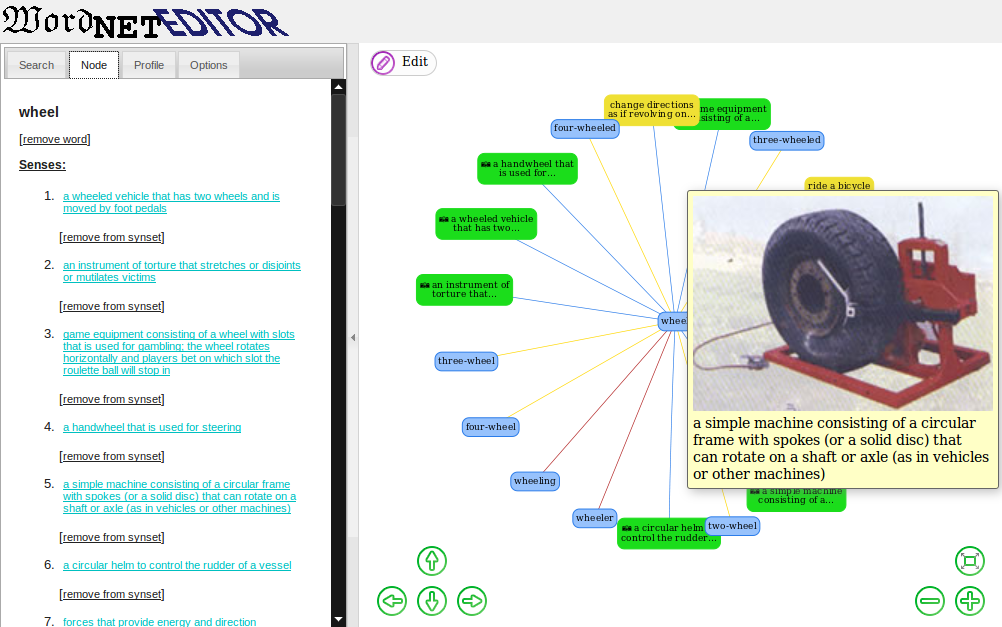
\includegraphics[width=1.0\textwidth]{wneditor.png}
					\caption{Ukázka rozhraní WordNET Editor: zvolený synset ve středu grafu a zobrazený obrázek k příbuznému synsetu}
					\label{fig:wneditor}
				\end{figure}

				Test chování tohoto rozhraní na mobilním zařízení nebyl proveden, jelikož je zjevné, že je určeno především k editacím a podle toho je také navrženo. Rozhraní poskytuje grafický náhled na strukturu dat, ale pro nevhodné kódování vztahů do barev a nezobrazovaní dostatečného množství informací je jeho ovládání neintuitivní. Nutno podotknout, že rozhraní tak, jak je vyobrazeno v \textcite{szymanski2007cooperative}, vypadá značně odlišně a například obsahuje pojmenované vztahy.

				Podle webové stránky projektu\td{cit http://wordventure.eti.pg.gda.pl/} je rozhraní vyvinuto s otevřeným zdrojem, pro jeho obdržení je však nutno kontaktovat vývojáře. Lze ale předpokládat jeho použitelnost i pro ostatní wordnety.

			\section{Cornetto Demo}
			\label{wnvis:cornetto}

				Cornetto Demo je prohlížeč pro nizozemský wordnet a jako jedno z mála dostupných webových aplikací kombinuje grafickou a textovou vizualizaci dat. To je dáno zřejmě mimo jiné tím, že Cornetto Demo není pouze rozhraním pro wordnet, ale kombinuje data ze dvou zdrojů. Jednak z Referentie Bestand Nederlands \parencite{martin2005referentie}, a jednak z nizozemského wordnetu. Referentie Bestand Nederlands je slovník obsahuji informace podobně strukturované jako FrameNet \parencite{fillmore2004framenet} spolu s rozšířením o kombinatorické chování slov v určitém významu \parencite{horak2008development}. 

				Rozhraní je rozděleno na tři moduly, základní vyhledávání, pokročilé vyhledávání a vizualizace synsetů. 

				Základní vyhledávání slouží k prostému vyhledávání lexikálních jednotek. Dotaz je možné základním způsobem omezovat či rozšiřovat, a to pomocí zástupných znaků (\ex{*}, \ex{?}\footnote{přičemž \ex{*} zastupuje posloupnost kterýchkoliv znaků, \ex{?} zastupuje jeden kterýkoliv znak}) a volby slovních druhů, v jakých se má výhledávat. \parencite{cornettoGettingStarted}

				Pokročilé vyhledávání umožňuje v nizozemském wordnetu najít lexikální jednotky, které mají společné specifické parametry. Jako kritéria pro vyhledávání lze zvolit kterékoliv kombinace všech příznaků, jež jsou ve wordnetu u lexikálních jednotek přítomny. Takto je možné například vyhledat všechna slovesa, která jsou řazena do domény tance a jsou označena jako archaická.  

				Pokud hledaný výraz či zvolená kritéria odpovídají některým lexikálním vyskytujícím se v databázi, je uživateli prezentován seznam nalezených jednotek, přes něž se lze prokliknutím dostat na detail té které jednotky. Detail je textovou reprezentací dostupných dat, tedy syntaktických a sémantických informací o vyhledaném slově (nutno podotknout, že značná část informací v této části zřejmě pochází spíše Referentie Bestand Nederlands, nikoliv z wordnetu) a hierarchického zařazení konceptu, do nějž slovo patří, ve wordnetu. Hierarchické zařazení je vyvedeno ve formě podobné tradičnímu znázornění adresářového stromu a obsahuje, zřejmě z úsporných důvodů, pouze přímé nadřazené a přímé podřazené koncepty a v rozhraní chybí úplné zobrazení cesty od kořene wordnetu k zobrazenému synsetu. I tak může strom být relativné dlouhý vzhledem k tomu, ze u obecných hyperonym bývá seznam hyponym rozsáhlý. 

				\begin{figure}[h]
					\centering
					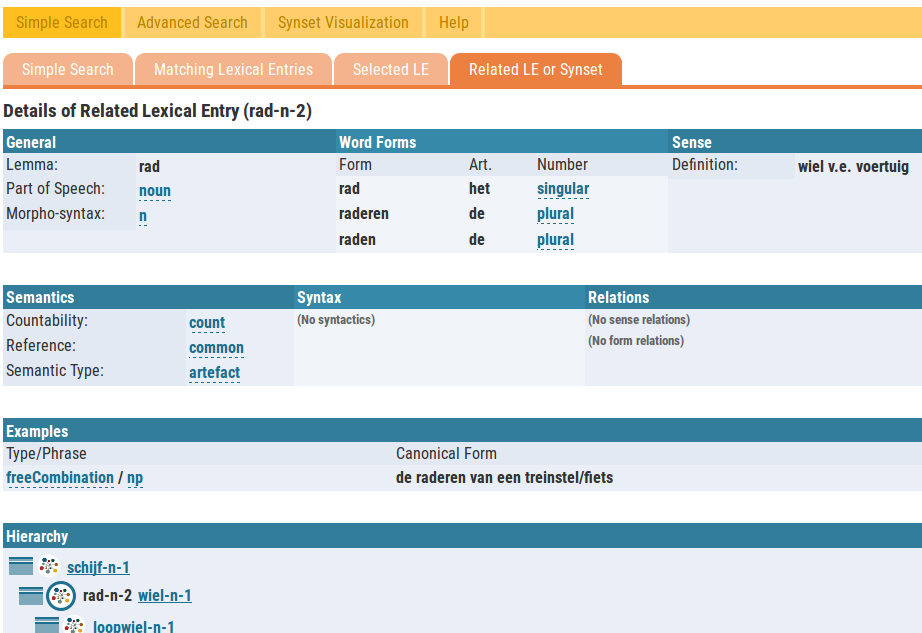
\includegraphics[width=1.0\textwidth]{cornetto-text1.png}
					\caption{Ukázka rozhraní Cornetto Demo: textová reprezentace dat}
					\label{fig:cornetto-text1}
				\end{figure}

				Z odkazů v hierarchii lze kliknutím na ikonu wordnetu u synsetu přejít do vizualizačního režimu, čímž se zobrazí grafické znázornění\td{vizualizuje vizualizační vizualizace, mwhahaha} daného synsetu. 

				Modul vizualizace synsetů je v praxi pouze pseudomodul, jelikož jeho vyhledávání se od základního vyhledávání liší pouze tím, že vybírá jeden výsledek vyhledávání a rovnou jej zobrazí v grafické znázornění. Který výsledek se má vybrat, je možné zvolit při inicializaci hledání. Je tak eliminována nutnost zvolit synset, otevřít jeho detaily a kliknout na výše zmíněnou ikonu, aby se uživatel dostal na grafické znázornění daného synset, jedná se však pouze o zkratku v rozhraní, jež nezavádání nic nového.

				Samotná vizualizace je realizovaná pomocí javascriptové knihovny d3 \parencite{BostockD3} a umožňuje uživateli prohlížet všechny synsety svázané nějakým vztahem s vyhledaným synsetem. Zobrazení rozlišuje syntaktické kategorie i sémantické vztahy barevně, přičemž vztahy jsou navíc ještě popsány slovně. Autoři použili rozšířený model vizualizace synsetů tak, že synset je představován uzlem, k němuž vede sémantický vztah, a z tohoto uzlu pak vedou nepojmenované hrany představující vazbu slovní formy na daný synset (tedy v zásadě vztah synonymie). Tento způsob je alternativní k zobrazení, v němž sémantické vztahy vedou k jednotlivým slovním formám a není tak na první pohled zřejmé, které navázané formy jsou součástí kterých synsetů. Zde použité zobrazení vhodně omezuje množství hran, které jsou nutné k vykreslení grafu, byť možná na úkor srozumitelnosti pro neznalého uživatele, jelikož body označující synset a hrany označující synonymii nejsou nijak označeny v grafu (pouze v legendě a při přejetí myší). Všechny uzly mají přiřazenou i vlastní legendu ve formě informační bubliny, která obsahuje například definici, příklady, slovní druh či identifikátory. Vizualizaci je možné kolečkem myši přibližovat a oddalovat a tažením myší se po zvětšeném grafu přesouvat. Funkčnost přibližování je možná poněkud diskutabilní, jelikož se při jejím použití nemění proporce zobrazovaných informací (cf. elektronické mapy na WWW, které při přiblížení sice zvětšují detail struktur, ale zachovávají velikost písmen v nápisech). Její smysl by v opačném případě tkvěl například v použití při vyhledání slov jako je \ex{plant}\footnote{niz. rostlina}, které mají velké množství hyponym, a tudíž jejich graf je nepřehledný až do rozměrů naprosté nepoužitelnosti (obrázek \ref{fig:wncorplant} na straně \pageref{fig:wncorplant}). Ovládání klávesnicí možné není.

				\begin{figure}[h]
					\centering
					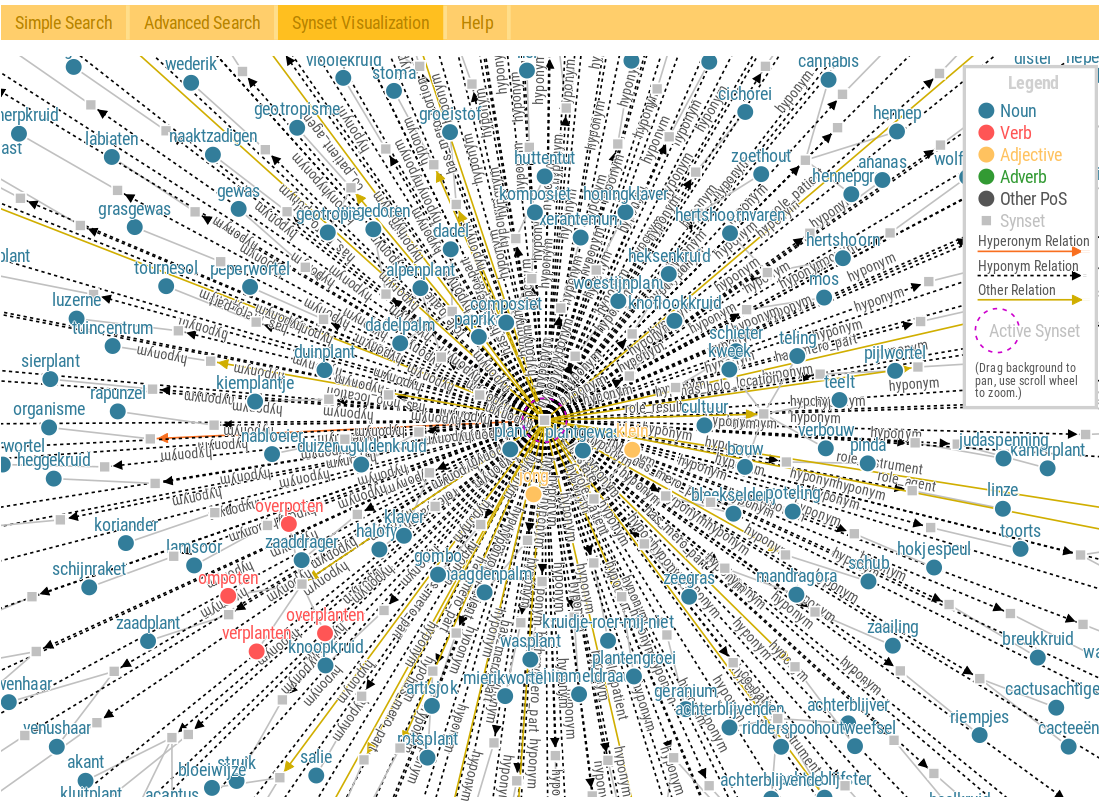
\includegraphics[width=1.0\textwidth]{wncorplant.png}
					\caption{Ukázka rozhraní Cornetto Demo: ilustrace přeplnění grafické reprezentace hyponymy u slova \ex{plant}}
					\label{fig:wncorplant}
				\end{figure}

				Rozhraní je neresponsivní, takže je na mobilním zařízení poněkud nepohodlné jej používat, byť to není nemožné. Šířka bloku s informacemi je natolik velká, že je nutné horizontálního rolování při čtení textu, což se považuje z hlediska použitelnosti webu za velmi negativní \parencite{nn2005scrollbar, richards2004web}. Reprezentace grafem je vzhledem k ovládání, které používá, ještě hůře použitelná. Dotyk prstem do plochy s vykresleným grafem je totiž zároveň interpretován jako rolování celé stránky a zároveň jako tažení plátna s grafem do stran, které je běžně prováděno tažením myší po plátně. Přibližování a oddalování grafu, nikoliv celé stránky, v testovacím prostředí nebylo možné vůbec, ale vzhledem k vlastnostem této funkce popsaným výše to použitelnost nijak neomezuje. Co v mobilním testovacím prostředí v podstatě nefungovalo, byly informační bubliny u slov, jež se normálně zobrazují nad slovy; zde se zobrazovaly zcela mimo inkriminované slovo a částečně mimo zobrazovanou plochu.

				Oproti základnímu rozhraní WordNet Search 3.1 přináší toto rozhraní přehlednější textovou reprezentaci dat spojenou s vizualizací vztahů vyhledaného synsetu. Textové rozhraní však zobrazuje poněkud omezené množství informací z wordnetu a soustřeďuje se především na data ze slovníku Referentie Bestand Nederlands. Vztahy mezi slovy jsou zobrazovány pouze v grafické reprezentaci dat, což vzhledem k její nepříliš vysoké použitelnosti na mobilních zařízeních s menší obrazovkou může být omezující. Rozhraní uchovává svůj stav podrobně v URL a umožňuje jej z ní plně obnovit.


			\section{WordVis}
			\label{vis:wordvis}

				WordVis je rozhraní zaměřené na vizualizaci dat princetonského WordNetu grafem. Sestává z vyhledávacího pole, levého sloupce s výběrem synsetů a plátnem, na němž je vykreslen graf vztahů zvoleného synsetu nebo slovní formy. 

				Ačkoliv to na první pohled uživateli nemusí být zřejmé, vizualizace funguje ve dvou režimech. Prvním je zobrazení slovní formy a synsetů, v nichž se tato slovní forma vyskytuje, druhé je zobrazení synsetu jako centrální jednotky a vztahů a slovních forem, které k danému synsetu patří. První zobrazení je užíváno například při prvotním zobrazení výsledků hledání. Vizualizace zobrazí ve středu grafu vyhledanou slovní formu a připojí k ní nepojmenovanými hranami synsety, jež danou slovní formu obsahují. Pokud pak uživatel zvolí kliknutím myší některý konkrétní synset, zobrazí se ve středu vizualizace jeho značka, k níž jsou připojeny pojmenovanými hranami představujícími sémantické vztahy další synsety. Stejně jako v prvním zobrazení, i v tomto se slovní formy náležející k určitému synsetu připojují nepojmenovanými hranami jako textové uzly. Pokud jedna slovní forma náleží k více synsetům (např. substantivum \ex{bicycle} a sloveso \ex{bicycle}), je v grafu její textový uzel pouze jednou a vedou od něj dvě nepojmenované hrany k náležitým synsetům. 

				Hrany mezi synsety jsou orientované (znázorněné jako šipky) a jejich k jejich pojmenování zvolil autor sémantické významy daných vztahů, tedy např. hyperonymie je značena slovem \textit{is}\footnote{angl. \textit{je}}; např. \ex{apple tree \textit{is} fruit tree}\footnote{angl. jabloň je ovocný strom}.

				Vyhledávací formulář umožňuje filtrování výsledků hledání podle slovních druhů a typů vztahu. Graf je navíc aktualizován v reálném čase podle toho, jak jsou podmínky filtrování uživatelem měněny. Nevýhodou však je absence funkcí \textit{vybrat vše} a \textit{nevybrat nic}, která je citelná zvláště v případě, že uživatel chce vybrat pouze jeden druh relace (kterých je mnoho, tudíž odebrání všech relací z výběru kromě jedné může být časově náročné). Hledání také nabízí funkci napovídání poté, co uživatel zadá několik znaků z počátku slova. To umožňuje vybrat hledané slovo z nabídky a ušetřit několik úhozů, což je zvláště užitečné u delších slov či pro uživatele, který nevyhledává ve svém rodném jazyce a není si jist pravopisem hledaného slova.

				\begin{figure}[h]
					\centering
					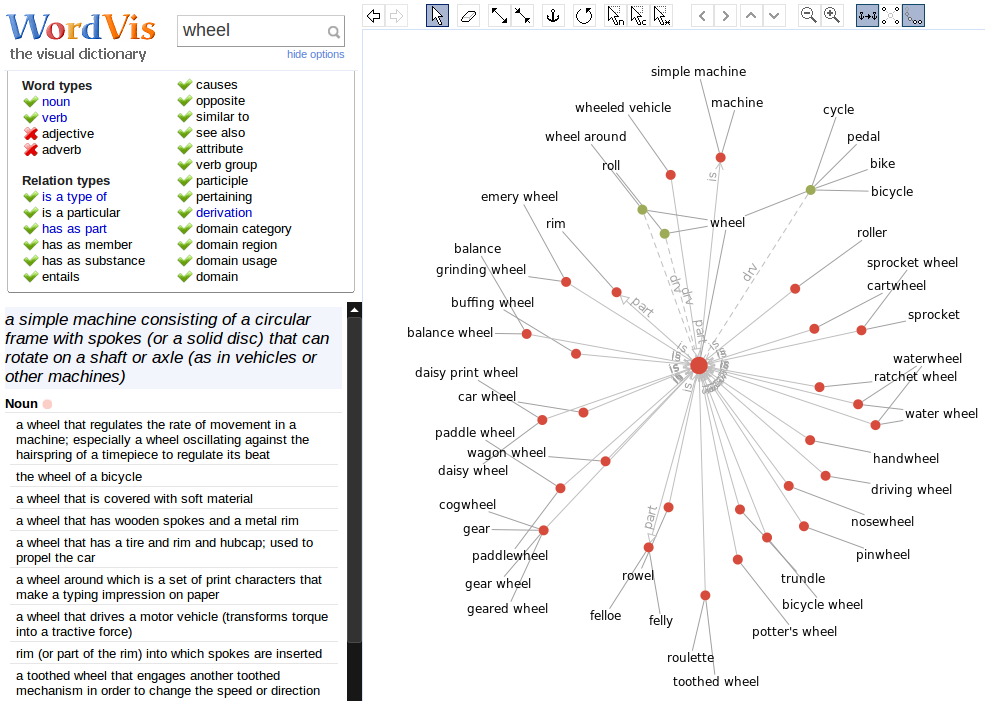
\includegraphics[width=1.0\textwidth]{wordvis.png}
					\caption{Ukázka rozhraní WordVis (po zvolení konkrétního vyhledaného synsetu)}
					\label{fig:wordvis}
				\end{figure}

				Technologicky je vizualizace řešena javascriptovou knihovnou, jež vykresluje graf na HTML5 plátně \parencite{w3schools2017htmlcanvas}. Uspořádání prvků na plátně je řešeno modelováním fyzikálních vlastností našeho světa. Jednotlivé uzly na plátně mají zadefinováno, že se navzájem odpuzují (podobně jako elektrony), naopak vazby mezi nimi fungují jako pružiny, jež mají nějakou ideální délku, v níž se snaží setrvávat. Díky těmto dvěma soupeřícím silám jsou body na plátně rozmístěny tak, aby využívaly prostor co nejúčinněji. Hrany navíc mohou mít zadanou preferovanou orientaci, což umožňuje orientovat například hyperonymní synsety směrem nahoru, hyponymní směrem dolu etc. \parencite{wordvis2010vercruysse} Vzhledem k tomu, že však zřejmě v prostředí neexistuje žádná penalizace za křížení hran, je relativně běžné, že se hrany překříží. To značně snižuje přehlednost výsledného grafu, vzhledem k tomu, že pak není jasné, zda jsou hrany překřízeny z nějakého hlubšího důvodu (například jedna slovní forma náležející k více synsetům), či nikoliv. Knihovna vykreslující graf umožňuje uživateli také modifikovat tažením jednotlivých uzlů myší, prodlužovat či zkracovat hrany a podobně. V aplikaci pro zobrazení dat z WordNetu toto nehraje přílišně zásadní roli a implementace této funkcionality je zřejmě dána tím, že knihovna je určena pro univerzálnější použití. \parencite{wordvis2010vercruysse}

				Rozhraní je neresponsivní a na mobilním zařízení je nutné k zajištění čitelnosti textů na stránce obsah přiblížit, což vede k nutnosti rolovaní jak vertikálnímu, tak horizontálnímu. Také není možné využít funkcionality přesouvání prvků na plátně, což ale při použití na vizualizaci dat z wordnetu není velkým omezením funkčnosti. Co se udržování stavu aplikace v URL týče, je implementováno pouze čtení parametru {\tt q} (od \textit{query}), zpětně do něj ale už zapisováno není. Odkazy na synsety na levé straně tento parametr obsahují, stejně tak jej lze zkopírovat přes kontextové menu pro každý uzel v rozhraní, takže teoreticky je možné obnovit kterýkoliv stav aplikace, byť dostupnost této funkcionality není příliš intuitivní.

				Přínos tohoto rozhraní tkví především v relativně přehledné vizualizaci dat princetonského WordNetu, nutno však podotknout, že pro některé své vlastnosti nemusí pro nezkušeného uživatele být zpočátku příliš intuitivní (např. zmíněné křížení hran).

				Na knihovně, na níž je toto rozhraní postaveno, stojí ještě některá další rozhraní k princetonskému WordNetu, například VisuWords\footnote{\url{http://www.visuwords.com/}, \url{https://www.linux.com/news/visuwords-wordnet-goes-graphical}} či Visual Thesaurus\footnote{\url{https://www.visualthesaurus.com}}. Ta nebyla do hodnocení v této práci zahrnuta, protože jsou funkčně podobná tomuto rozhraní.

			\section{sloWTool}
			\label{vis:slowtool}

				Rozhraní sloWTool bylo vyvinuto pro potřeby slovinského wordnetu, jenž je založen na princetonském WordNetu a vznikl skombinováním několika zdrojů, například Wikipedie, dvojjazyčných slovníků či paralelních korpusů. Je víceúčelovým nástrojem, který umožňuje textovou reprezentaci, vizualizaci a editaci dat z wordnetu. Tvůrcům sloužilo k revizím slovinského wordnetu po jeho rozšiřování automatickými nástroji. \parencite{fivser2012slownet} Cílem při vývoji tohoto rozhraní podle \textcite{fivser2011visualizing} bylo překonat nevýhody tehdejších dostupných rozhraní a vyvinout nástroj, který by mezi jiným umožňoval prohlížení i editaci, spolupráci mnoha autorů včetně anonymních editací (záměr tvůrců byl využít náhodných návštěvníků k opravování chyb, jež ve wordnetu naleznou) či možnost jednoduché registrace uživatelů. Mezi dalšími podmínkami byla možnost přidávání dalších wordnetů do systému a s tím spojená schopnost rozhraní zobrazovat vícejazyčná data. V neposlední řadě se autoři v kontextu tehdejších nástrojů také snažili zaměřit na platformní nezávislost a přenositelnost rozhraní. 

				Rozložení stránky je vzdáleně podobné tomu u základního oficiálního rozhraní k princetonskému WordNetu, a to v tom smyslu, že neobsahuje relativně rozšířený levý sloupec na výběr synsetů, ale jednotlivé významy, které jsou nalezeny po zadaní hledané slovní formy do vyhledávacího pole, seskupuje do sekcí v hlavním bloku s textovou reprezentací dat. Vyhledávací pole podporuje napovídání existujících významů, což může usnadnit práci s rozhraním. V textové reprezentací rozhraní zobrazuje zřejmě všechny dostupné informace o synsetech, tedy se chová podobně jako základní rozhraní princetonského WordNetu, je-li nastaveno tak, aby nefiltrovalo žádné informce. U jednotlivých vztahů, v nichž je daný synset přítomen, pak je možné kliknutím otevřít synset nacházející se pomyslně na druhé straně daného vztahu (např. \ex{bicykle} má meronymum \ex{sedlo}, takže lze otevřít detail synsetu \ex{sedlo}). To trpí stejným neduhem, jako základní rozhraní princetonského WordNetu, to jest, že lze ve smyčce otevírat nadřazený a podřazený synset a stále se zanořovat do smyčky hlouběji. To je nejen nesmyslné, ale zároveň to v implementaci tohoto rozhraní postupně může začít zpomalovat rychlost reakcí prohlížeče pro nadměrné množství uzlů v DOM\footnote{document object model}.

				Po levé straně se nachází lišta s ikonami odkazujícími na dalšími moduly, které se otevírají v emulacích nových oken (v témže panelu). Mezi tyto moduly patří mimo jiné i pokročilé hledání, vizualizace a nápověda. 

				Pokročilé hledání funguje podobně jako u ostatních rozhraní, tedy umožňuje používat zástupné znaky (\ex{*} a \ex{?}), filtrovat slovní druhy, nebo vyhledávat v jiných polích než jsou slovní formy patřící do synsetů (například v definicích či podle identifikátoru synsetu). 

				Vizualizace, modul z hlediska této práce nejpodstatnější, je určen k zobrazení grafické interpretace vztahů vyhledanýho synsetů. Na rozdíl od ostatních rozhraní tato vizualizace zobrazuje všechny vyhledané synsety (s kořenem grafu označeným jako \textit{search}\footnote{hledání}) a neumožňuje jejich filtrování. Také nepodporuje zřejmě žádnou formu interakce kromě přesouvání prvků na plátně a zvýraznění příslušného synsetu v hlavním bloku textové reprezentace poté, co je na něj (nebo jeho členskou slovní formu) ve vizualizaci kliknuto. Pokud uživatel potřebuje zobrazit vizualizaci jednoho konkrétního synsetu, je nucen použít pokročilé vyhledávání a vyhledat daný synset nejlépe podle jeho identifikátoru, který je vždy unikátní. Vizualizace je zatížena také dalšími problémy, jako jsou nedostatečné možnosti přizpůsobování velikosti zobrazovací plochy (zvětšování okna je podporováno, ale plátno s grafem zůstává konstantně velké), občasnou desynchronizací obsahu vizualizace s výsledky hledání, náročností na uživatelovo technické vybavení počítače (především výpočetní jednotku) a značnou nepřehledností způsobenou nedostatečně či nevhodně řešenou penalizací překrývání prvků na zobrazovací ploše. 

				\begin{figure}[h]
					\centering
					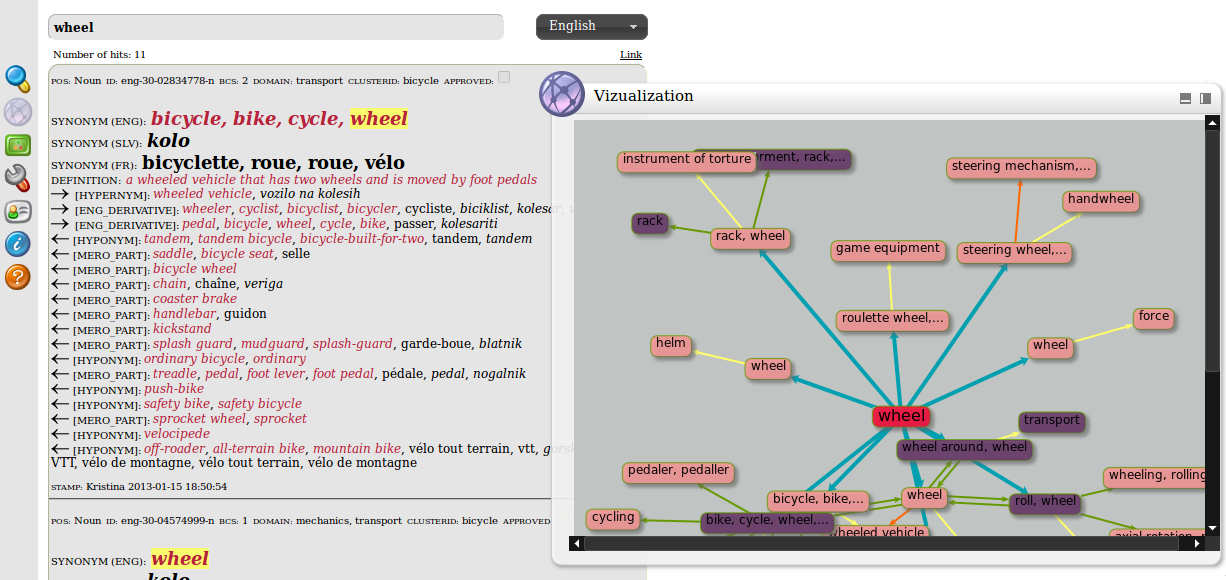
\includegraphics[width=1.0\textwidth]{slowtool.png}
					\caption{Ukázka rozhraní sloWTool (s otevřenou grafickou vizualizací)}
					\label{fig:slowtool}
				\end{figure}

				Rozhraní je svými možnostmi zprostředkování informací z wordnetu poměrně inovativní, reálná použitelnost ovšem trpí zmíněnými nedostatky a odchyluje jej tím od původního záměru autorů, který minimálně zčásti zůstává nenaplněn. Je sice pravdou, že \textit{s aplikací je možné pracovat v každém moderním přihlížeči, ať už na počítači, tabletu, či dokonce mobilním telefonu} \parencite{fivser2011visualizing}, nutno ale podotknout, že rozhraní je zcela neresponsivní a jeho ovládací prvky jsou zcela nevhodné pro ovládání na menší obrazovce a dotykem.

				Stav aplikace lze do jisté míry uložit pomocí odkazu \textit{Link}, který vede na adresu, z níž lze obnovit hledané slovo (konfiguraci otevřených nástrojů však už nikoliv).

				Navzdory všem nedostatkům této aplikace je dlužno uznat, že se svou univerzalitou a funkcionalitou značně přibližuje rozhraní, které je praktickým cílem i této práce.

				SloWtool bylo vytvořeno pod licencí Creative Commons\footnote{\url{https://creativecommons.org/licenses/by-nc-sa/3.0/}} a jeho zdrojový kód je dostupný na platformě pro aplikace s otevřeným zdrojem Launchpad\footnote{\url{https://launchpad.net/slowtool}}.

			\section{BabelNetXplorer}
			\label{vis:babel}

				BabelNet je rozsáhlý projekt vícejazykové sémantické sítě, který čerpá data z více zdrojů. Záměrem autorů bylo při tvorbě této sémantické sítě 
				% poskytnout vědecké komunitě i široké veřejnosti volně dostupný multilinguální zdroj provázaných informací a soubor nástrojů, které umožní s těmito informacemi pracovat. 
				eliminovat základní faktory definující nevýhody tehdejších (a potažmo i aktuálních) mezinárodních projektů zabývajících se sémantickými sítěmi. Těmi jsou manuální tvorba dat, které sítě konstituují, a s tím související nerovnoměrnost množství dat přes jednotlivé jazyky. Jazyky s vysokou hustotou zdrojů, jakým je například angličtina, tak ve výsledku mají více dat i v sémantické síti. Autoři BabelNetu se pokusili tento problém překonat kombinací několika metod, jejichž společným jmenovatelem je automatizace. Informace o významech jsou v BabelNetu doplňovány z Wikipedie, která je podle autorů díky mnohačetným zásahům expertů z různých oborů ve výsledku přesným a informarčně bohatým zdrojem. Druhá důležitá metoda, zaměřující se především na nerovnoměrnost dat v různých jazycích, je automatický překlad zdrojů. \parencite{navigli2010babelnet}

				BabelNetXplorer je webové grafické rozhraní vytvořené pro vizualizaci dat z BabelNetu. \cite{navigli2012babelnetxplorer} uvádějí, že rozhraní slouží k vizualizaci vztahů pro slova nalezená v BabelNetu a ilustrují vzhled rozhraní dvěma snímky obrazovky. V době vzniku této práce však rozhraní BabelNetXploreru vypadá výrazně odlišně, což je vzhledem k tomu, že od vzniku práce \cite{navigli2012babelnetxplorer} uběhlo pět let, pochopitelné. V této práci bude z evidentních důvodů rozebrána použitelnost a funkcionalita současného rozhraní.

				Rozhraní obsahuje klasicky vyhledávací pole, vedle něhož se nacházejí rozbalovací menu, v nichž si uživatel může vybrat, ve kterém jazyce chce vyhledávat a, případně, do kterého jazyke chce slovo přeložit. Po úspěšném dokončení vyhledávání jsou uživateli zobrazeny odkazy na jednotlivé synsety v seznamu, který není nepodobný ostatním rozhraním. Podstatným rozdílem však je, že se v něm zobrazují i ilustrační obrázky, které, byť nejsouce vždy velmi informativní, mohou napomoci uživateli v orientaci, který synset jej zajímá. 

				V detailu synsetu, který se zobrazí po kliknutí na příslušný odkaz, je uživateli zobrazen seznam slovních forem, které k daném synsetu náleží, jeho definice (s možností zobrazit i jeho definice nejen z daného wordnetu, v němž uživatel vyhledává, ale i z Wikipedie a dalších zdrojů), jeho případný překlad a sémantické vztahu, do nichž tento synset náleží. K disposici má uživatel i možnost zobrazit si daný synset paralelně v dalších jazycích pomocí nabídky pod vyhledávacím polem (viditelné na snímku obrazovky \ref{fig:babelxplorer} na straně \pageref{fig:babelxplorer}). Níže na stránce jsou uživateli prezentovány informace z dalších zdrojů napojených na BabelNet, jako jsou obrázky, překlady, odkazy na Wikipedii, etc. a odkaz na vizuální reprezentaci sémantických vztahů otevřeného synsetu. 

				\begin{figure}[h]
					\centering
					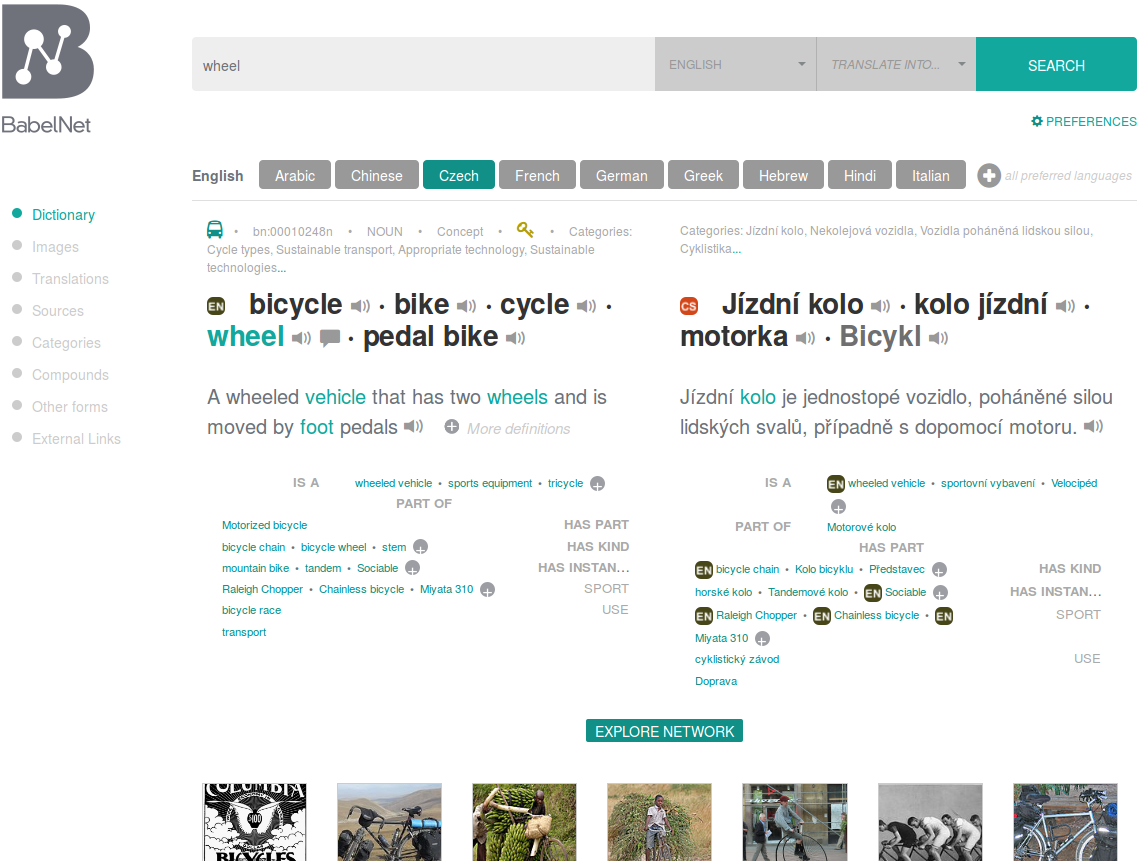
\includegraphics[width=1.0\textwidth]{babelxplorer.png}
					\caption{Ukázka rozhraní BabelXplorer (detail synsetu v textové reprezentaci)}
					\label{fig:babelxplorer}
				\end{figure}

				Vizuální reprezentace je řešena tradičním hvězdicovitým grafem, který má dva režimy. Jeden zobrazuje vedle textových názvů jednotlivých synsetů přítomných v grafu i jejich zástupné obrázky, druhý je čistě textový a, nutno podotknout, značně přehlednější. Uzly reprezentující synsety jsou provázány barevně odlišenými hranami, kde barvy značí druh vztahů, který dva synsety spojuje. Uzly jsou klikatelné, přičemž po kliknutí na některý z příbuzných synsetů se zobrazí tento synset a opět hvězdicovitě další synsety, s nimiž je zkoumaný synset provázán některým ze vztahů. Při najetí korsorem myši na určitý synset se zobrazí jeho detail; tyto informační bubliny jsou však vázány na pozici kursoru myši a nelze tak kursorem najet do detailu tak, aby bylo možné kliknout na odkazy, které jsou v informační bublině obsaženy, a dostat se tak na textovou reprezentaci daného synsetu. Zdá se tedy, že není možné přejít z grafické reprezentace do textové.

				Poněkud nešťastně je řešen design vizualizace, jelikož jednak není možné graf přibližovat a oddalovat, a jednak pokud uživatel nenajede na konkrétní synset kursorem myši, graf se samovolně neustále otáčí, což ztěžuje orientaci v něm.

				Rozhraní všeobecně responsivní, textová reprezentace je dobře použitelná i na mobilním rozhraní s malou obrazovkou. Grafická reprezentace je však omezena na větší obrazovky, jelikož v ní není možné graf posouvat po obrazovce, a tudíž jeho značná část (byť se částěčně přizpůsobuje zobrazovací ploše), zřejmě v závislosti na velikosti obrazovky zařízení, zůstává uživateli skryta.

				V době vzniku této práce mělo rozhraní dvě verze, z nichž jedna byla označana jako \textit{živá beta}, druhá jako \textit{současná (3.7)}, avšak při testování nebyly zjištěny zásadní rozdíly mezi těmito verzemi. Nutno ovšem podotknout, že na testovacím desktopovém prohlížeči vykazovala verze beta minoritní chyby v rozložení stránky.

		\chapter{Vizulizace v aplikačním prostředí Java}

			Java je objektově orientovaný programovací jazyk, který je zaměřený na to, aby měl co nejméně závislostí na konkrétním operačním systému a technickém vybavení počítače, jak jen to je možné. To je výhodné zejména kvůli tzv. konceptu WORA (\textit{write once, run anywhere}, tedy napiš jednou, spusť kdekoliv), protože to znamená, že skompilované programy napsané v Javě lze spustit na jakémkoliv stroji, který podporuje Javu. Takto skompilované programy se spouští v aplikačním prostředí zvaném Java Virtual Machine\footnote{virtuální stroj Javy} (JVM), jež vytváří uniformní prostředí pro běh aplikací. Výhodou Javy tedy je velká přenositelnost programů v tomto jazyce napsaných, jelikož jednou skompilovaný kód lze spustit na různých operačních systémech a zařízeních. Nevýhodou je, že si uživatel, který chce program v Javě spustit, musí nainstalovat aplikační prostředí Javy (JVM). 

			Java je velmi oblíbená pro vývoj aplikací, které fungují podle modelu klient--server, což je uspořádání, v němž data má uložená centrální server, k nemuž se připojují uživatelské klienty, odesílají mu své požadavky a uživatelům zobrazují vrácená data. Na podobném principu může fungovat i rozhraní pro wordnet, pokud jsou data wordnetu uložena na serveru.

			Vizualizace vytvořené pro prostředí Java nemá příliš smysl hodnotit z hlediska responsivity, jelikož a priori nejsou vytvářena pro mobilní zařízení (až na výjimky, které nebylo možné zhodnotit z důvodu jejich nedostupnosti v době vzniku této práce). Co však bráno v potaz být může je jejich schopnost přizpůsobit se velikosti obrazovky. Jakkoliv tento parametr může se zdát být samozřejmým, ukázalo se, že ne všechna rozhraní jsou na různé velikosti obrazovek osobních počítačů přizpůsobena.

			\section{wnbroswer}

				\begin{figure}[ht]
					\centering
					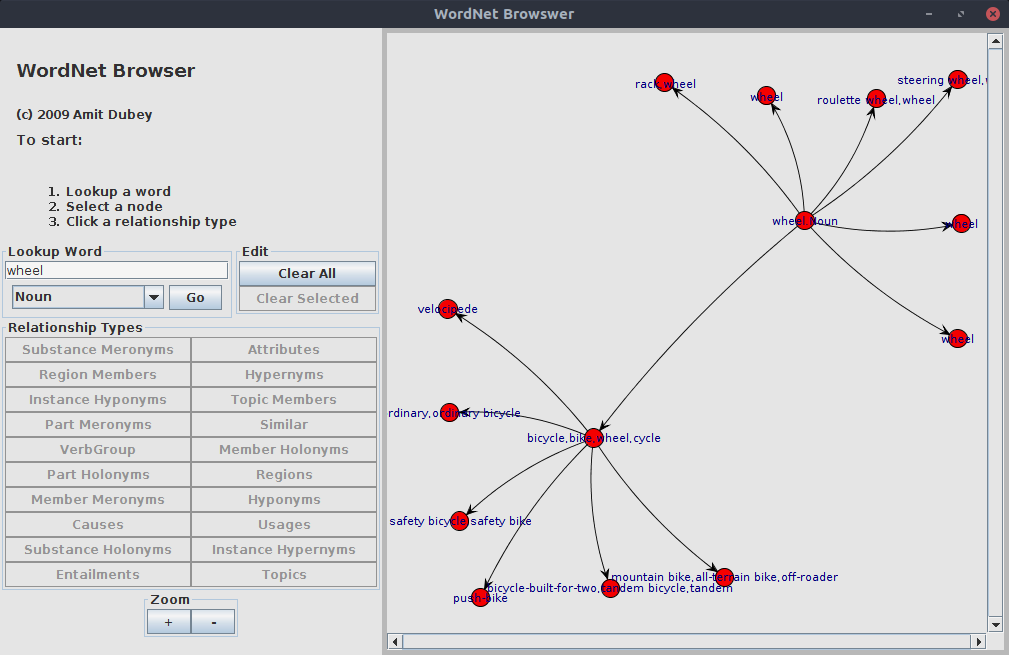
\includegraphics[width=1.0\textwidth]{wnwordnetbrowswer.png}
					\caption{Ukázka rozhraní wnbroswer}
					\label{fig:wnwordnetbrowswer}
				\end{figure}

				Rozhraní wnbroswer\footnote{sic erat scriptum} je určeno k prezentaci dat z princetonskému WordNetu, které pracuje pouze s grafovou grafickou reprezentací. Bylo vytvořeno pro reprezentaci dat z WordNetu ve verzi 3.0 a vyšší a vyžaduje lokální instalaci dat. Rozhraní je zřejmě svázáno se vznikem rumunského wordnetu \parencite{fivser2011visualizing}. Sestává z vyhledávacího pole, volby, mezi kterými syntaktickými kategoriemi se má vyhledávat, a selektoru na typy vazeb, jež mají být zobrazeny. Po úspěšném vyhledání konkrétního slova se zobrazí graf konceptuálně podobný grafu z rozhraní sloWTool, tedy ve středu je uzel reprezentující hledaný výraz, z něhož vedou hrany k jednotlivým synsetům, jež danou slovní formu obsahují. 

				Grafická reprezentace je interaktivní, tedy na ní lze zvolit, jaký druh sémantického vztahu se má zobrazit, a lze tak u každého uzlu postupně zobrazit všechny synsety, které jsou s ním provázány; toho lze docílit buď přes kontextové menu, nebo přes volby vztahů v levém sloupci rozhraní, v němž se mimo jiné nachází i vyhledávací pole. Rozhraní zobrazuje i detaily zvoleného synsetu (po kliknutí na daný synset), takže až na technické informace typu číslo významu a podobně je schopno zobrazovat všechna dostupná data.

				Jakkoliv velikost okna s aplikací měnit lze, velikost plochy pro vykreslování grafu zůstává neměnné velikosti, lze tedy v terminologii webových aplikací říci, že je neresponsivní, jelikož se nedokáže přizpůsobit velikosti obrazovky zařízení uživatele.

				Aplikaci je možné používat bez připojení k Interetu, jelikož spoléhá na data WordNetu nainstalovaná lokálně. 

				Poněkud komicky působí fakt, že rozhraní má tři různé názvy: wnbroswer (hlavní nadpis stránky projektu), WordNet Browswer (titulek okna aplikace) a wnbrowser (ostatní výskyty). 

			\section{Treebolic}

				\begin{figure}[ht]
					\centering
					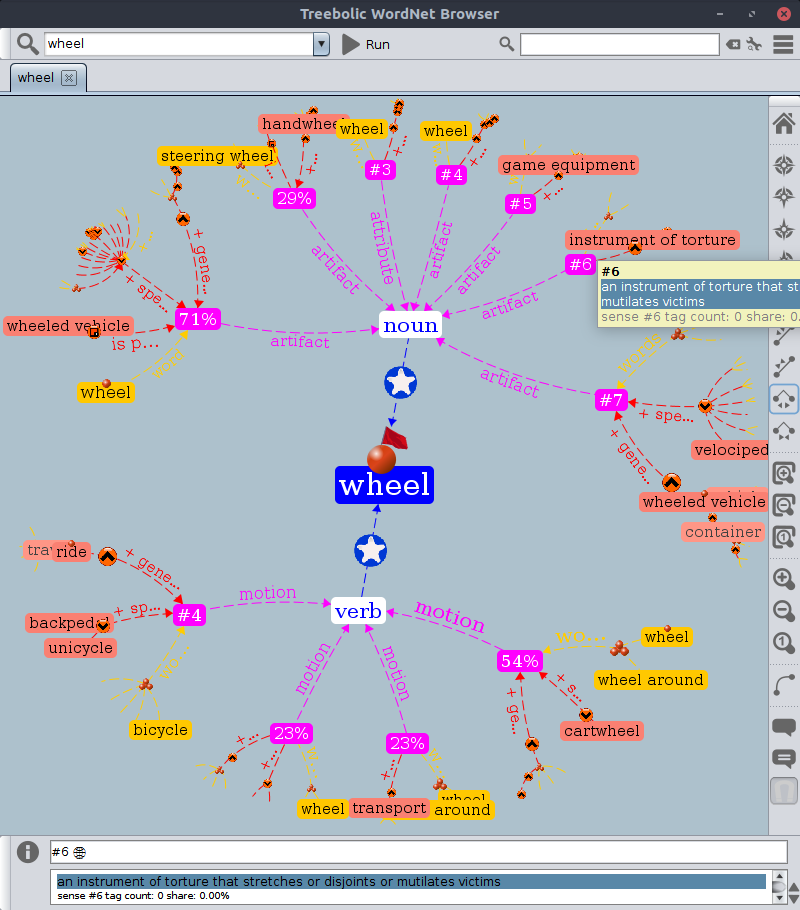
\includegraphics[width=1.0\textwidth]{wntreebolic.png}
					\caption{Ukázka rozhraní Treebolic (se zobrazenou informační bublinou na synsetu)}
					\label{fig:wntreebolic}
				\end{figure}

				Treebolic je aplikace určená k zobrazování hierarchických dat v hyperobilicke reprezentaci, která zajišťuje, že důležitá data v centru obrazovky jsou zobrazena uživateli ve větším měřítku, než data na okrajích grafu. Reprezentaci si lze představit jako plochu zobrazenou přes čočku. 

				Zobrazení používá model prezentující vše, co je nalezeno k hledanému slovu, tedy při úspěšném vyhledání výsledků se veprostřed vizualizace zobrazí reprezentace vyhledávání, s níž jsou hranami provázáany všechny nalezené synsety. Oproti ostatním zde popisovaným prostředím navíc seskupuje tyto synsety podle slovního druhu, tedy zavádí další metakategorii v zobrazení, což přispívá k přehlednosti zobrazení. 

				Co jí naopak ubírá, jsou poněkud kryptické ikony sémantických vztahů, jejichž význam je sice popsán na hraně, kde jsou dané ikony umístění, popřípadě je možno jej odhalit pomocí nabídky \textit{Info} v kontextovém menu po kliknutí pravým tlačítkem danou ikonu, ale při prvním setkání se toto řešení nezdá být příliš ergonomickým (mimo jiné proto, že duplikuje informace). Ne zcela evidentní jsou také číselné a procentuální údaje v místě uzlů se synsety. Uživatel se sice díky řešení, které používá konexe hranami ze synsetů k členským slovním formám, dozví, o který synset jde (díky oněm členským slovním formám), ale význam zmíněných údajů zůstává skryt. Výhdoou je barevné kódování významů jednotlivých hran. Barvy jsou navíc editovatelné v nastavení, takže teoreticky rozhraní vyhoví i osobám se zhoršeným vnímáním barev.

				Aplikace byla vyvinuta i pro Android (jakkoliv v rámci této práce netestována), tudíž lze říci, že jistým zprostředkovaným způsobem splňuje požadavky na responsivitu.

				Aplikaci je možné používat bez připojení k Interetu, jelikož spoléhá na data WordNetu nainstalovaná lokálně.

				Teoretický přínos této implementace spočívá v pohledu na stratifikaci důležitosti vizualizovaných dat. Idea hyperbolického zobrazení, rozvinutá dále především v oblasti ovladatelnosti, by mohl být správným krokem prezentace dat ve větším množství, než je schopna obrazovka (a potažmo zorné pole) uživatele pojmout.

			\section{VisualBrowser}

				Verze aplikace VisualBrowser testovaná v rámci této práce neprokázala dostatečnou intuitivitu a funkčnost, aby její vlastnosti mohly být dále rozebrány. 

		\chapter{Desktopové aplikace}

			Desktopové aplikace jsou takové aplikace, které jsou nativně určeny pro běh na operačním systému uživatelova počítače. Nativně spouštěná aplikace je, ať už přímo, či nepřímo, závislá na programových vlastnostech operačního systému daného stroje, stejně jako zprostředkovaně na jeho technickém vybavení. Přístupy k distribuci desktopových aplikací jsou v zásadě dva; první, z evidentních důvodů běžný především pro operační systém Windows, spočívá v distribuci již skompilovaných binárních souborů, které zajistí instalaci daného programu do systému a uživateli zbývá jen příslušný program spustit. Druhý způsob, běžný spíše pro různé linuxové distribuce, je založený na distribuci souborů obsahujících zdrojový kód programu, přičemž uživatel je nucen, má-li zájem program používat, si binární spustitelný soubor skompilovat. Druhý způsob pro programátora skýtá zásadní výhodu v tom, že se nemusí zajímat o prostředí, na němž bude koncový uživatel jeho program provozovat, protože kompilace programu pro všechny dostupné konfigurace (kombinace progamového a technickéh vybavení koncového uživatele) je náročná na zdroje. \parencite{Elizabeth2015} Pro onoho koncového uživatele však slyne druhá varianta tou nevýhodou, že kompilace programového vybavení vyžaduje z jeho strany netriviální usilí a znalosti o vlastním systému. 

			V rámci rozhraní určených pro zprostředkování dat z wordnetů jsou desktopové aplikace nejméně zastoupeny. Je tomu pravděpodobně proto, že jsou nejnáročnější na vývoj, zvláště mají-li být dostupné ze všech majoritních desktopových platforem. Dalším důvodem může být fakt, že často bývá zvolen model klient--server, pro který jsou vhodnější spíše aplikace v Javě \parencite[13]{gosling1995java} a webová rozhraní.

			\section{Artha}

				\begin{figure}[h]
					\centering
					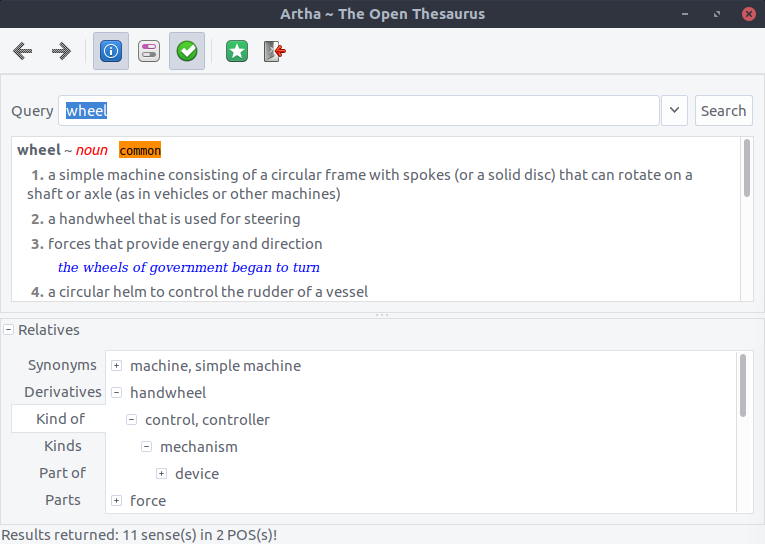
\includegraphics[width=1.0\textwidth]{wnartha-ubuntu.png}
					\caption{Ukázka rozhraní aplikace Artha}
					\label{fig:wnartha-ubuntu}
				\end{figure}

				Artha je multiplatformí thesaurus založený na WordNetu 3.0 \parencite{ramaswamy2012}. Grafické prostředí aplikace je vytvořeno v GTK\footnote{multiplatformní soubor nástrojů pro tvorbu grafických rozhraní (\url{https://www.gtk.org/})}, takže umožňuje (minimálně na testovací konfiguraci, tedy operační systém Ubuntu 16.04) komfortní práci. Je možno ji nainstalovat z repozitářů (tedy nevyžaduje náročnou kompilaci), což je pro koncového uživatele velmi pozitivní. Dle dokumentace je k disposici instalátor i na operační systém Windows\footnote{\url{https://www.microsoft.com/en-us/windows/}}. O Apple macOS\footnote{\url{https://www.apple.com/lae/macos}} se dokumentace nezmiňuje. Funguje bez připojení k Internetu a zobrazení je zaměřeno především na zobrazení významů synsetů (význam jsa reprezentován definicemi). Problémem je ukládání stavů aplikace, který se projevuje na nepříliš propracované funkcionalitě možnosti kroku zpět (na předchozí vyhledávání). Pokud například uživatel dvojklikne na slovo v definici, Artha se jej pokusí\footnote{selže, pokud uživatel vybere před dvojklikem více slov} přesměrovat na definici tohoto slova ve WordNetu, ale při kroku zpět už mu zobrazí slovo které hledal \textit{před} slovem, z něhož se dostal na \textit{současnou} definici. Oproti základnímu rozhraní WordNetu nabízí Artha větší pohodlí v podobě desktopové offline aplikace, což pro uživatele například znamená, že není při používání tohoto rozhraní závislý na připojení k Internetu.

				Artha zobrazuje data čistě textově (ve smyslu, že nenabízí žádnou formu vizualizace), přičemž rozhraní dělí na dvě části, a to nalezené synsety a sémantické vztahy, které se k danému synsetu vážou (ilustrováno na snímku obrazovky \ref{fig:wnartha-ubuntu} na straně \pageref{fig:wnartha-ubuntu}). 

			\section{GoldenDict}
 		
 				\begin{figure}[h]
					\centering
					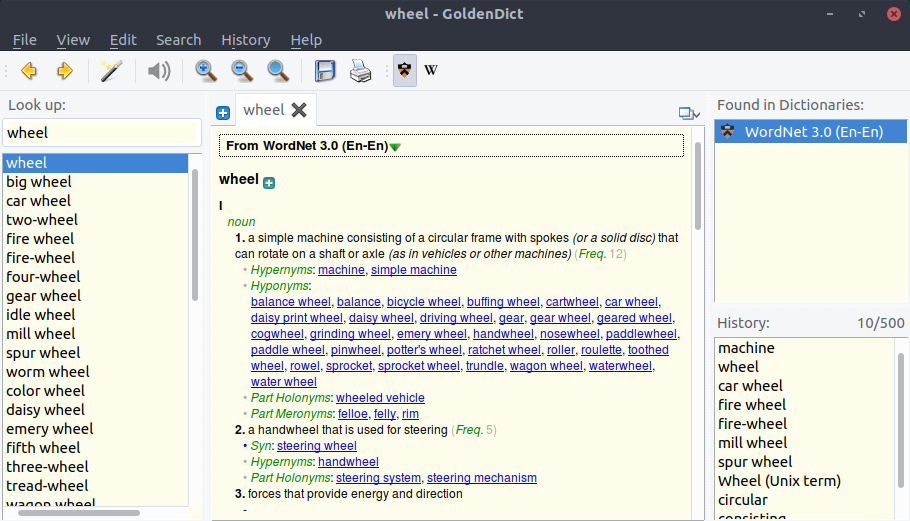
\includegraphics[width=1.0\textwidth]{wngoldendick-ubuntu.png}
					\caption{Ukázka rozhraní aplikace GoldenDict}
					\label{fig:wngoldendick-ubuntu}
				\end{figure}

				Podobně jako Artha funguje GoldenDict, který, byvše univerzálnějším rozhraním pro více lexikografických zdrojů, byl testován jen ve své verzi pro WordNet. GoldenDict zobrazuje čistě textovou reprezentaci umožňující kliknutím zobrazit detaily jednotlivých synsetů. Slovníková data si obstarává aplikace sama, takže uživatel nemusí podstupovat instalaci dat princetonského WordNet (která může být netriviální, protože například pro Windows neposkytují oficiální webové stránky instalátor pro data WordNetu ve verzi 3). Zároveň však rozhraní umožňuje přidávat další slovníky a v základu umožňuje zobrazovat výsledku hledání z Wikipedie. 

				Rozhraní obsahuje levý sloupec pro zobrazování výsledků hledání a společně s hlavní plochou pro zobrazování detailů synsetu se chová podobně jako ostatní rozhraní (ilustrováno na snímku obrazovky \ref{fig:wngoldendick-ubuntu} na straně \pageref{fig:wngoldendick-ubuntu}). Aplikace udržuje historii hledání, umožňuje hledat slova z definic synsetů pomocí dvojkliku kursorem myši a dává uživateli k disposici relativně široké možnosti konfigurovatelnosti. Její rozhraní se dobře přizpůsobuje velikosti obrazovky (potažmo okna).

				Grafické rozhraní aplikace GoldenDict je postaveno na Qt\footnote{\url{https://www.qt.io/ui/}} a pro zobrazování dat z webu používá vykreslovací jádro WebKit\footnote{\url{https://webkit.org/}}. \parencite{goldendict2016}


		\chapter{Shrnutí přehledu rozhraní a vyplývající závěry o vhodném rozhraní k sémantickým sítím}

			% z hlediska pouzitelnosti byva lepsi webovy rozhrani, bo to uzivatel nemusi instalovat (some fuken links for that)
			% java je sice kchul, ale porad ji musi mit uzivatele nainstalovanou, asi lidi moc nemaji (applety jsou uplne k nicemu uz, FF to prestal podporovat)
			% drtiva vetsina rozhrani neni responsivni, coz je problem, kdyz vetsina lidi pouziva web z mobilu: http://bgr.com/2016/11/02/internet-usage-desktop-vs-mobile/
			% je potreba rozhrani, ktery bude webovy, vypadat konsistentne na vsech zarizenich a bude splnovat, co se od nej ocekava (designove) - co se ocekava od WN browseru? dunno, but it's important - https://conversionxl.com/why-simple-websites-are-scientifically-better/

			Rozhraní v přehledu prezentovaném v této práci byla hodnocena dle různých aspektů odpovídajícím účelu a provedení dané třídy rozhraní. Nejpodrobněji byla hodnocena webová rozhraní. U těch byla jako největší společný nedostatek identifikována nedostatečná responsivita, což vede k tomu, že uživatel dané rozhraní nemůže (nebo může velmi omezeně) používat na mobilním zařízení. To v době, kdy počet uživatelů přistupujících k webovým službám přes mobilní zařízení je vyšší než počet těch, kteří k nim přistupují pomocí klasických stolních počítačů \parencite{Heisler2016}, aplikaci značně diskriminuje. Z podobného důvodu jsou v nevýhodě také rozhraní vytvořená pro aplikační prostředí Java a v ještě větší míře aplikace vytvořené přímo pro operační systémy stolních počítačů. 

			Aplikace vytvořené v Javě jsou sice teoreticky spustitelné i na některých mobilních operačních systémech (zejména Android\footnote{\url{https://android.stackexchange.com/questions/63710/can-you-run-normal-java-programs-on-android}}, u ostatních je podpora omezená či žádná\footnote{\url{http://stackoverflow.com/questions/15501477/can-windows-phone-support-java}, \url{http://www.iphonefaq.org/archives/9731}, \url{http://stackoverflow.com/questions/1193524/can-we-run-java-applictions-on-iphone} inter alia}), prakticky je jejich použitelnost vzhledem k jejich designu grafického rozhraní omezena ale také výhradně na stolní počítače. 

			Pro některé aplikace vyvinuté v Javě byly vytvořeny tzv. aplety Java\footnote{\url{https://nlp.fi.muni.cz/projekty/visualbrowser/applet/index.html}}, ale vzhledem k tomu, že některé silně rozšířené webové prohlížeče tento druh zásuvných modulů už vůbec nepodporují \parencite{MozzilaFoundation2017}, je jejich použití značně omezené a do budoucnosti lze předpokládat plošnou nepoužitelnost. 

			Rozhraní závislá na platformě (operačním systému, případně aplikačním rozhraní) mají navíc tu nevýhodu, že uživatel nalezená data nemůže jednoduše sdílet například se svými kolegy (od toho u webových rozhraní hodnocené reflektování stavu aplikace v adresním řádku prohlížeče). 

			Z výše uvedeného je zřejmé, že je potřeba rozhraní, které bude použitelné univerzálně na všech platformách, a zároveň bude implementovat funkcionalitu všeobecně očekávanou u rozhraní pro wordnet. Tou je jednak textová prezentace dat a k ní dodatečná vizualizice ve formě grafu. Ideální rozhraní by také mělo splňovat designové požadavky moderních webových aplikací na přístupnost, tedy například nepředpokládat určitou velikost obrazovky uživatelova zařízení či ctít zásady vizuální přístupnosti (konstrastní barevné kódování, nepřekrývání textových prvků na obrazovce etc.). Je samozřejmě evidentní, že grafická prezentace dat nemůže být přizpůsobena velikosti obrazovky mobilního zařízení, mají-li být textové prvky čitelné a zároveň zachované rozložení prvků, může však být alespoň zajištěno, že funkcionalita posouvání zobrazovací plochy dotykem (u dotykových zařízení) není znemožněna funkcionalitou svázanou s prvky na obrazovce (jak tomu často bývá u implementací grafů synsetů, jejichž uzly je možné tažením myší přesouvat po zobrazovací ploše). 

			Kýžené rozhraní by také mělo splňovat požadavky na vizuální atraktivitu, aby se uživatelé cítili komfortně při práci s takovým rozhraním. Aspekty vizuálně komfortního rozhraní jsou do značné míry subjektivní, zdá se však, že uživatelé očekávají jistou prototipičnost designového konceptu od webové stránky s určitým účelem \parencite{walker2013simple, tuch2012role}. Studie \parencite{tuch2012role} také potvrzuje, že uživatelé pozitivně vnímají webové stránky s nízkou komplexitou, což může u implementace rozhraní wordnetu být problémem, jelikož takové rozhraní inherentně musí poskytovat velké množství informací. Cílem tedy je zobrazované informace vhodně strukturovat tak, aby uživatel měl pocit, že danou stránku zná a ví, kde na ní co najde, a necítil se zahlcen množstvím informací. Detaily designu takové aplikace jsou rozebrány v [zatím neexistující kapitole o tom, jak ty cypovinu píšu]. 

	\part{Praktická část: rozhraní k sémantické síti}

		\chapter{Design rozhraní}

			\section{Textová prezentace}


			\section{Grafická prezentace}


		\chapter{Použité technologie}

			\section{HTML}

			\section{CSS}

			\section{JavaScript}

			\section{JSON}


 
	% \begin{spacing}{1.05}
	\printbibliography[]
	% \printbibliography[title={Seznam literatury}]
	% \bibliographystyle{alpha}
	% \bibliography{bibliografie}
	% \end{spacing}

	\addcontentsline{toc}{chapter}{Bibliografie}

\end{document}